% Template for PLoS
% Version 3.4 January 2017
%
% % % % % % % % % % % % % % % % % % % % % %
%
% -- IMPORTANT NOTE
%
% This template contains comments intended 
% to minimize problems and delays during our production 
% process. Please follow the template instructions
% whenever possible.
%
% % % % % % % % % % % % % % % % % % % % % % % 
%
% Once your paper is accepted for publication, 
% PLEASE REMOVE ALL TRACKED CHANGES in this file 
% and leave only the final text of your manuscript. 
% PLOS recommends the use of latexdiff to track changes during review, as this will help to maintain a clean tex file.
% Visit https://www.ctan.org/pkg/latexdiff?lang=en for info or contact us at latex@plos.org.
%
%
% There are no restrictions on package use within the LaTeX files except that 
% no packages listed in the template may be deleted.
%
% Please do not include colors or graphics in the text.
%
% The manuscript LaTeX source should be contained within a single file (do not use \input, \externaldocument, or similar commands).
%
% % % % % % % % % % % % % % % % % % % % % % %
%
% -- FIGURES AND TABLES
%
% Please include tables/figure captions directly after the paragraph where they are first cited in the text.
%
% DO NOT INCLUDE GRAPHICS IN YOUR MANUSCRIPT
% - Figures should be uploaded separately from your manuscript file. 
% - Figures generated using LaTeX should be extracted and removed from the PDF before submission. 
% - Figures containing multiple panels/subfigures must be combined into one image file before submission.
% For figure citations, please use "Fig" instead of "Figure".
% See http://journals.plos.org/plosone/s/figures for PLOS figure guidelines.
%
% Tables should be cell-based and may not contain:
% - spacing/line breaks within cells to alter layout or alignment
% - do not nest tabular environments (no tabular environments within tabular environments)
% - no graphics or colored text (cell background color/shading OK)
% See http://journals.plos.org/plosone/s/tables for table guidelines.
%
% For tables that exceed the width of the text column, use the adjustwidth environment as illustrated in the example table in text below.
%
% % % % % % % % % % % % % % % % % % % % % % % %
%
% -- EQUATIONS, MATH SYMBOLS, SUBSCRIPTS, AND SUPERSCRIPTS
%
% IMPORTANT
% Below are a few tips to help format your equations and other special characters according to our specifications. For more tips to help reduce the possibility of formatting errors during conversion, please see our LaTeX guidelines at http://journals.plos.org/plosone/s/latex
%
% For inline equations, please be sure to include all portions of an equation in the math environment.  For example, x$^2$ is incorrect; this should be formatted as $x^2$ (or $\mathrm{x}^2$ if the romanized font is desired).
%
% Do not include text that is not math in the math environment. For example, CO2 should be written as CO\textsubscript{2} instead of CO$_2$.
%
% Please add line breaks to long display equations when possible in order to fit size of the column. 
%
% For inline equations, please do not include punctuation (commas, etc) within the math environment unless this is part of the equation.
%
% When adding superscript or subscripts outside of brackets/braces, please group using {}.  For example, change "[U(D,E,\gamma)]^2" to "{[U(D,E,\gamma)]}^2". 
%
% Do not use \cal for caligraphic font.  Instead, use \mathcal{}
%
% % % % % % % % % % % % % % % % % % % % % % % % 
%
% Please contact latex@plos.org with any questions.
%
% % % % % % % % % % % % % % % % % % % % % % % %

\documentclass[10pt,letterpaper]{article}
\usepackage[top=0.85in,left=2.75in,footskip=0.75in]{geometry}

% amsmath and amssymb packages, useful for mathematical formulas and symbols
\usepackage{amsmath,amssymb}

% Use adjustwidth environment to exceed column width (see example table in text)
\usepackage{changepage}

% Use Unicode characters when possible
\usepackage[utf8x]{inputenc}

% textcomp package and marvosym package for additional characters
\usepackage{textcomp,marvosym}

% cite package, to clean up citations in the main text. Do not remove.
\usepackage{cite}
% Use nameref to cite supporting information files (see Supporting Information section for more info)
% \usepackage{nameref,hyperref}

% line numbers
\usepackage[right]{lineno}

% ligatures disabled
\usepackage{microtype}
\DisableLigatures[f]{encoding = *, family = * }

% color can be used to apply background shading to table cells only
\usepackage[table]{xcolor}

% array package and thick rules for tables
\usepackage{array}

% create "+" rule type for thick vertical lines
\newcolumntype{+}{!{\vrule width 2pt}}

% create \thickcline for thick horizontal lines of variable length
\newlength\savedwidth
\newcommand\thickcline[1]{%
  \noalign{\global\savedwidth\arrayrulewidth\global\arrayrulewidth 2pt}%
  \cline{#1}%
  \noalign{\vskip\arrayrulewidth}%
  \noalign{\global\arrayrulewidth\savedwidth}%
}

% \thickhline command for thick horizontal lines that span the table
\newcommand\thickhline{\noalign{\global\savedwidth\arrayrulewidth\global\arrayrulewidth 2pt}%
\hline
\noalign{\global\arrayrulewidth\savedwidth}}

%%%%%%%%%% Our stuff %%%%%%%%%%%%%%%%

% \graphicspath{ {artwork/} }

\usepackage{caption}
\usepackage{graphicx}
\graphicspath{ {artwork/} }
\usepackage{amsthm}
\usepackage{array}
\usepackage{booktabs}

% \usepackage{caption}
\usepackage{subcaption}
\usepackage{multirow}
\usepackage{tabularx}
\usepackage{afterpage}
\usepackage{rotating}
\usepackage{setspace}
\usepackage{soul}

\usepackage[acronym,toc,shortcuts]{glossaries}


% Don't include all these in the glossary:
% Instead pick the central ones by hand and explain
\newacronym{A1}{A1}{primary auditory cortex}
\newacronym{ICA}{ICA}{independent component analysis}
\newacronym{IT}{IT}{inferotemporal cortex}
\newacronym{LDR}{LDR}{linear dimensionality reduction}
\newacronym{LGN}{LGN}{lateral geniculate nucleus}
\newacronym{mPFC}{mPFC}{medial prefrontal cortex}
\newacronym{MST}{MST}{medial superior temporal area}
\newacronym{MSTd}{MSTd}{dorsal subregion of the medial superior temporal area}
\newacronym{MT}{MT}{middle temporal area}
\newacronym{NMF}{NMF}{nonnegative matrix factorization}
\newacronym{NSC}{NSC}{nonnegative sparse coding}
\newacronym{PCA}{PCA}{principal component analysis}
\newacronym{PFC}{PFC}{prefrontal cortex}
\newacronym{RDDR}{RDDR}{reinforcement-driven dimensionality reduction}
\newacronym{RF}{RF}{receptive field}
\newacronym{RLVM}{RLVM}{rectified latent variable model}
\newacronym{RSC}{RSC}{retrosplenial cortex}
\newacronym{SNN}{SNN}{spiking neural network}
\newacronym{STA}{STA}{spike-triggered average}
\newacronym{STDP}{STDP}{spike-timing dependent plasticity}
\newacronym{STDPH}{STDPH}{spike-timing dependent plasticity and homeostatic synaptic scaling}
\newacronym{STNMF}{STNMF}{spike-triggered nonnegative matrix factorization}
\newacronym{V1}{V1}{primary visual cortex}
\newacronym{VIP}{VIP}{ventral intraparietal area}
\newacronym{VPS}{VPS}{visual posterior sylvian area}
\newacronym{WTA}{WTA}{winner-take-all}

\usepackage{hyphenat}
\hyphenation{high-di-men-sion-al}

%  Add  todonotes package for commenting (xargs enables newcommandx for making comments for each person)
\usepackage{xargs}
\usepackage[textsize=scriptsize]{todonotes}\reversemarginpar
\setlength{\marginparwidth}{5cm}
% Comment style for mike, blue background + border
\newcommandx{\mikeNote}[2][1=]{\todo[linecolor=black,backgroundcolor=blue!25,bordercolor=blue,#1]{#2 ---Mike}}
% Comment style for kris, red background + border.
\newcommandx{\krisNote}[2][1=]{\todo[linecolor=black,backgroundcolor=red!25,bordercolor=red,#1]{#2 ---Kris}}
% Comment style for emily, green background + border.
\newcommandx{\emilyNote}[2][1=]{\todo[linecolor=black,backgroundcolor=green!25,bordercolor=green,#1]{#2 ---Emily}}
% Comment style for jeff, orange background + border.
\newcommandx{\jeffNote}[2][1=]{\todo[linecolor=black,backgroundcolor=orange!25,bordercolor=orange,#1]{#2 ---Jeff}}
% Comment style for nik, orange background + border.
\newcommandx{\nikNote}[2][1=]{\todo[linecolor=black,backgroundcolor=yellow!25,bordercolor=yellow,#1]{#2 ---Nik}}


%% Get rid of these ugly boxes around links
\usepackage[colorlinks=true, hidelinks]{hyperref}
\hypersetup{
    linkcolor={black!50!black},
    citecolor={black!50!black},
    urlcolor={black!80!black}
}

%%%%%%%%%%%%%%%%%%%%%%%%%%%%%%%%%%%%%%



% Remove comment for double spacing
%\usepackage{setspace} 
%\doublespacing

% Text layout
\raggedright
\setlength{\parindent}{0.5cm}
\textwidth 5.25in 
\textheight 8.75in

% Bold the 'Figure #' in the caption and separate it from the title/caption with a period
% Captions will be left justified
\usepackage[aboveskip=1pt,labelfont=bf,labelsep=period,justification=raggedright,singlelinecheck=off,font={small}]{caption}
\renewcommand{\figurename}{Fig}


% Use the PLoS provided BiBTeX style
% \usepackage[authoryear]{natbib}
\bibliographystyle{plos2015}


% Remove brackets from numbering in List of References
\makeatletter
\renewcommand{\@biblabel}[1]{\quad#1.}
\makeatother

% Leave date blank
\date{}

% Header and Footer with logo
\usepackage{lastpage,fancyhdr,graphicx}
\usepackage{epstopdf}
\pagestyle{myheadings}
\pagestyle{fancy}
\fancyhf{}
\setlength{\headheight}{27.023pt}
\lhead{
\includegraphics[width=2.0in]{PLOS-submission.eps}}
\rfoot{\thepage/\pageref{LastPage}}
\renewcommand{\footrule}{\hrule height 2pt \vspace{2mm}}
\fancyheadoffset[L]{2.25in}
\fancyfootoffset[L]{2.25in}
\lfoot{\sf PLOS}

\usepackage{pbox,ragged2e}

%% Include all macros below

\newcommand{\revise}[1]{\textcolor{blue}{#1}}

%% END MACROS SECTION


\begin{document}
\vspace*{0.2in}

% Title must be 250 characters or less.
\begin{flushleft}
{\Large
\textbf\newline{Sparse coding and dimensionality reduction in the brain} % Please use "sentence case" for title and headings (capitalize only the first word in a title (or heading), the first word in a subtitle (or subheading), and any proper nouns).
}
\newline
% Insert author names, affiliations and corresponding author email (do not include titles, positions, or degrees).
\\
Michael Beyeler\textsuperscript{1,2*\Yinyang},
Emily L. Rounds\textsuperscript{1\Yinyang},
Kristofor D. Carlson\textsuperscript{3},
Nikil Dutt\textsuperscript{1},
Jeffrey L. Krichmar\textsuperscript{1}
\\
\bigskip
\textbf{1} University of California, Irvine, CA, USA
\\
\textbf{2} University of Washington, Seattle, WA, USA
\\
\textbf{3} Sandia National Laboratories\dag, Albuquerque, NM, USA
\\
\bigskip

% Insert additional author notes using the symbols described below. Insert symbol callouts after author names as necessary.
% 
% Remove or comment out the author notes below if they aren't used.
%
% Primary Equal Contribution Note
\Yinyang These authors contributed equally to this work.

% Additional Equal Contribution Note
% Also use this double-dagger symbol for special authorship notes, such as senior authorship.
% \ddag These authors also contributed equally to this work.

% Current address notes
% \textcurrency Current Address: Dept/Program/Center, Institution Name, City, State, Country % change symbol to "\textcurrency a" if more than one current address note
% \textcurrency b Insert second current address 
% \textcurrency c Insert third current address

\dag Sandia National Laboratories is a multiprogram laboratory managed and operated by National Technology and Engineering Solutions of Sandia, LLC, for the U.S. Department of Energy's National Nuclear Security Administration under contract DE-NA0003525.

% Group/Consortium Author Note
% \textpilcrow Membership list can be found in the Acknowledgments section.

% Use the asterisk to denote corresponding authorship and provide email address in note below.
* mbeyeler@uw.edu

\end{flushleft}
% Please keep the abstract below 300 words
\section*{Abstract}
Supported by recent computational studies, sparse coding and dimensionality reduction are emerging as a ubiquitous coding strategy  across brain regions and modalities, allowing neurons to achieve \acf{NSC} by efficiently encoding high-dimensional stimulus spaces using a sparse and parts-based population code. Reducing the dimensionality of complex, multimodal sensory streams is critically important for metabolically constrained brain areas to represent the world.
\revise{In this article, we demonstrate that a wide variety of neuronal responses}
ranging from \revise{sensory} processing, to spatial navigation, to memory systems
\revise{can be understood as an emergent property of \acf{NSC},
an efficient population coding scheme
based on dimensionality reduction and sparse coding.}
\revise{This finding suggests that \acs{NSC} might be a general principle
to which many neuronal computations adhere.
In addition, \acs{NSC} might provide a useful theoretical framework under which
to understand the often complex and nonintuitive response properties
of neurons in brain areas far removed from sensory input.}

% Furthermore, 
% \revise{we discuss potential biophysical mechanisms that}
% % show that specific forms of synaptic plasticity and homeostatic modulation 
% may underlie its implementation,
% \revise{and} propose that \acs{NSC} is an organizing principle in the nervous system.
% and has implications for machine learning
% \mikeNote{We don't really talk about machine learning anymore, do we?}
% and sparse computation.


% Please keep the Author Summary between 150 and 200 words
% Use first person. PLOS ONE authors please skip this step. 
% Author Summary not valid for PLOS ONE submissions.   
\section*{Author summary}
Brains face the fundamental challenge of processing, storing, and representing high-dimensional stimuli using patterns of neural activity. One potential approach to addressing this challenge is to reduce the number of variables required to represent a particular stimulus space (i.e., dimensionality reduction).
We review compelling evidence that a wide range of neuronal responses can be understood as an emergent property of \acf{NSC}---a form of efficient population coding due to dimensionality reduction and sparsity constraints.
\revise{The success of these models warrants further investigation.
In fact, we propose that \acs{NSC} is an organizing principle for neuronal computation.}
% we posit that biological synaptic plasticity and homeostasis mechanisms can carry out the same function as \acs{NSC}.

\linenumbers


\section*{Introduction}
\label{sec:introduction}
Brains face the fundamental challenge of 
processing, storing, and representing high-dimensional stimuli
using patterns of neural activity.
To support complex patterns of behavior, 
populations of interconnected neurons implement 
a rich repertoire of linear and nonlinear operations on their synaptic inputs
and vary their signaling properties based on context and experience
\cite{Koch1999}.

However, neuronal information processing is complicated
by strict constraints on metabolic cost---50\% of the 
mammalian brain's energy consumption is believed to be associated with 
neuronal signaling \cite{Laughlin2001, Lennie2003}---and the 
widespread existence of anatomical bottlenecks 
\cite{Kempermann2002,BarGad2003_Review,Babinsky1993}.
These bottlenecks often force the information
stored in a large number of neurons
to be compressed into an orders of magnitude smaller population
of downstream neurons;
for example, storing information from 100 million photoreceptors 
in 1 million optic nerve fibers,
or resulting in a $10 - 10,000$ fold convergence from cortex to the basal ganglia
\cite{BarGad2003_Review}.
To operate efficiently within these constraints,
it has been suggested that the nervous system improves 
efficiency by reducing (and in some cases minimizing) the resources
required to implement a given task \cite{LaughlinSejnowski2003}.

One potential approach to addressing this challenge is to
reduce the number of signals required to transmit information in the network.
\textbf{Sparse coding} schemes (see Glossary),
in which information is represented by the activity of a small
proportion of neurons in a population,
have been shown to greatly increase energy efficiency 
\cite{Foldiak1990,Field1994,LevyBaxter1996}.
An extreme example is the so-called \emph{local code}
where each unique event or `context' is encoded by a single active neuron
or `grandmother cell' \cite{RollsTreves1990}
(illustrated in the left column of Fig.~\ref{fig:sparse-parts}A).
Although local codes lead to low energy expenditure, 
they also suffer from low \textbf{representational capacity},
because they allow a population of $N$ neurons to encode at most $N$ contexts.
On the other hand, a \emph{dense code}
represents each context by the combined activity
of all neurons in the population
(Fig.~\ref{fig:sparse-parts}A, right column).
Dense codes lead to high representational capacity
(at $M$ activity levels, allowing for $M^N$ contexts to be encoded),
but also suffer from neuronal cross talk,
because every neuron is involved in every context.
Alternatively, sparse codes
(Fig.~\ref{fig:sparse-parts}A, center column)
can be described as a trade-off between the benefits and
drawbacks of dense and local codes 
\cite{SpanneJorntell2015,Foldiak1990},
leading to relatively low energy expenditure while maintaining a 
relatively high representational capacity.
The level of sparsity required to minimize energy expenditure can be determined
by weighing the cost of maintaining a neuron at rest against the extra cost
of sending a signal:
when signals are relatively expensive, it is best to distribute a few of them
among a large number of cells (local code); but
when cells are expensive, it is more efficient to use few cells
and have all of them participate in the encoding of the signal (dense code)
\cite{RollsTreves1990,Laughlin2001}.


\begin{figure}[h]
	\centering
	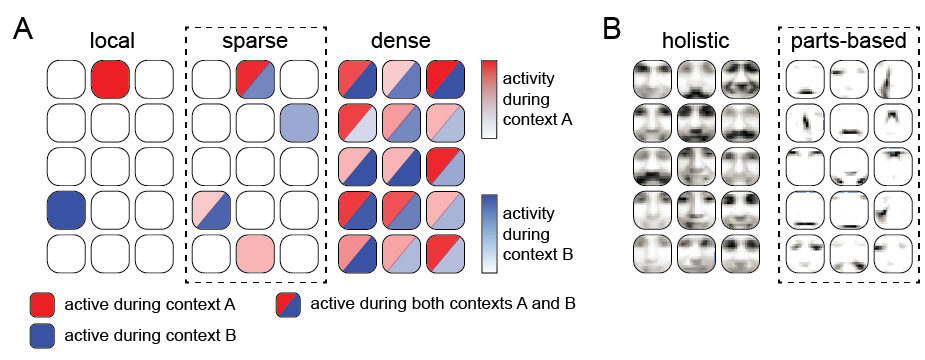
\includegraphics[width=\textwidth]{fig-rev1-sparse}
    \caption{\Acf{NSC} promotes population codes that are both sparse and parts-based.
    \textbf{\emph{A}},
    	   Hypothetical activity in a population of neurons
           during presentation of two different external stimuli (`contexts').
           A sparse code is a trade-off between a local code
           (where a context is represented by the activity of a single neuron,
           and different contexts are represented by different neurons), and a
           dense code (where all neurons are active and their combined activity is
           used to encode each context).
           Dense codes possess great memory capacity, but suffer from cross talk
           among neurons, whereas local codes do not suffer from interference
           but also have no capacity for generalization
           (adapted from \cite{SpanneJorntell2015}).
     \textbf{\emph{B}},
           In a holistic representation of faces, 
           individual neurons in the population
           respond themselves to faces as a whole \cite{TanakaFarah1993},
           whereas in a parts-based representation
           individual neurons explicitly encode individual face components
           \cite{Palmer1977},
           such as the eyes, nose, and mouth
           (adapted from \cite{LeeSeung1999}).}
	\label{fig:sparse-parts}
\end{figure}


Another approach is to reduce the number of
variables required to represent a particular stimulus space;
a process known as
\textbf{dimensionality reduction}.
Dimensionality reduction methods have proved useful in elucidating neural mechanisms
that depend on how the responses of multiple neurons covary,
including odor discrimination in the olfactory system \cite{Broome2006,Koulakov2011},
the selection and integration of sensory inputs 
in the prefrontal cortex \cite{Mante2013},
and the ability of premotor cortex 
to prepare movements without executing them \cite{Kaufman2014}.

In brain areas far removed from sensory input,
neurons typically encode several behaviorally relevant parameters
simultaneously \cite{Rigotti2013,Park2014,PaganRust2014,PougetSejnowski1997},
allowing for multifaceted representations of high-dimensional stimulus spaces.
For example, a population of neurons tasked with encoding human faces
might opt to represent each individual face as a combination of a set of
standard faces (Fig.~\ref{fig:sparse-parts}B, left column).
In such a \textbf{holistic representation} of faces \cite{TanakaFarah1993},
each individual neuron would itself respond to a face as a whole
(i.e., a face `template')
without explicitly representing individual face components,
and an arbitrary face could be represented by 
combining different face templates
(e.g., by adding 10\% of template 1 to 20\% of template 2
and subtracting 30\% of template 3).
On the other hand, faces can also be represented as a combination
of individual face components, such as eyes, noses, and mouth,
in what is known as a \textbf{parts-based representation}
(Fig.~\ref{fig:sparse-parts}B, right column) \cite{Palmer1977}.
Both approaches allow for representing arbitrary faces as a combination of
neural activity, but have drastically different consequences on the
set of stimulus features each neuron responds to.
Although visual information from the eyes, nose, and mouth would of course be
included in a holistic face representation,
that information would not be explicitly represented as structural units
in their own right \cite{TanakaFarah1993}.
Linear combinations of holistic components often involve complex cancellations
between positive and negative contributions,
and thus lack the intuitive meaning of adding parts to form a whole.
In contrast, a parts-based representation allows for only nonsubtractive
combinations of stimulus features \cite{Palmer1977}.
Although the relevant stimulus dimensions are often not known \emph{a priori},
several sophisticated mathematical techniques exist that
allow us to discover these representations directly from experimental data
\cite{Brunton2016,CunninghamYu2014,PillowSimoncelli2006,Sharpee2014,Gao2017}.

In this article, we demonstrate that a variety of neuronal responses
can be understood as an emergent property of efficient population coding
based on dimensionality reduction and sparse coding.
Specifically, we review computational evidence
from data analyses and computer simulations arguing that \ac{NSC}, 
a combination of \textbf{\ac{NMF}}
\cite{PaateroTapper1994,LeeSeung1999} 
and sparse coding,
can generate sparse and parts-based embeddings of
high-dimensional stimulus spaces
that resemble neuronal population responses in a 
wide variety of brain regions.
This introduces the possibility that \ac{NSC} might
be a general principle to which many neuronal computations adhere.
Furthermore, \ac{NSC} might provide a useful theoretical framework under which
to understand the often complex and nonintuitive response properties of neurons
in brain areas far removed from sensory input.

\section*{Nonnegative sparse coding (NSC) as a modern variant of the efficient coding hypothesis}

\subsection*{Efficient coding}

The fundamental principle of \textbf{efficient coding}
is that a sensory system is
adjusted to the specific statistics of the natural environment from which
it encodes and transmits information
\cite{Barlow1961,Attneave1954,Linsker1990,LouieGlimcher2012}.
\revise{Efficiency, in this context, is an information-theoretic term 
that should not be confused with `minimizing energy expenditure'.
Instead, a sensory pathway is treated as a noisy communication channel, where 
the goal is to maximize the rate at which information can be reliably transmitted
by minimizing the redundancy between representational units.}

Early theories of efficient coding
\cite{Barlow1961,Attneave1954}
were developed based on the visual system.
Attneave \cite{Attneave1954} pointed out that there is a significant
degree of redundancy in natural visual images due to correlations in both
the spatial and temporal domains
(for a recent review, see \cite{SimoncelliOlshausen2001}).
For example, the luminance values of a pair of pixels
separated by a fixed distance in a natural image
are likely to be highly correlated
(Fig.~\ref{fig:ech}A).
These statistical regularities constrain the images a visual system
is likely to encounter to a tiny fraction of the set of all
possible images.
It was therefore argued that the visual system should not
waste resources on processing arbitrary images,
but instead use statistical knowledge
about its environment to represent the relevant input space 
as economically as possible.


\begin{figure}[h]
	\centering
% 	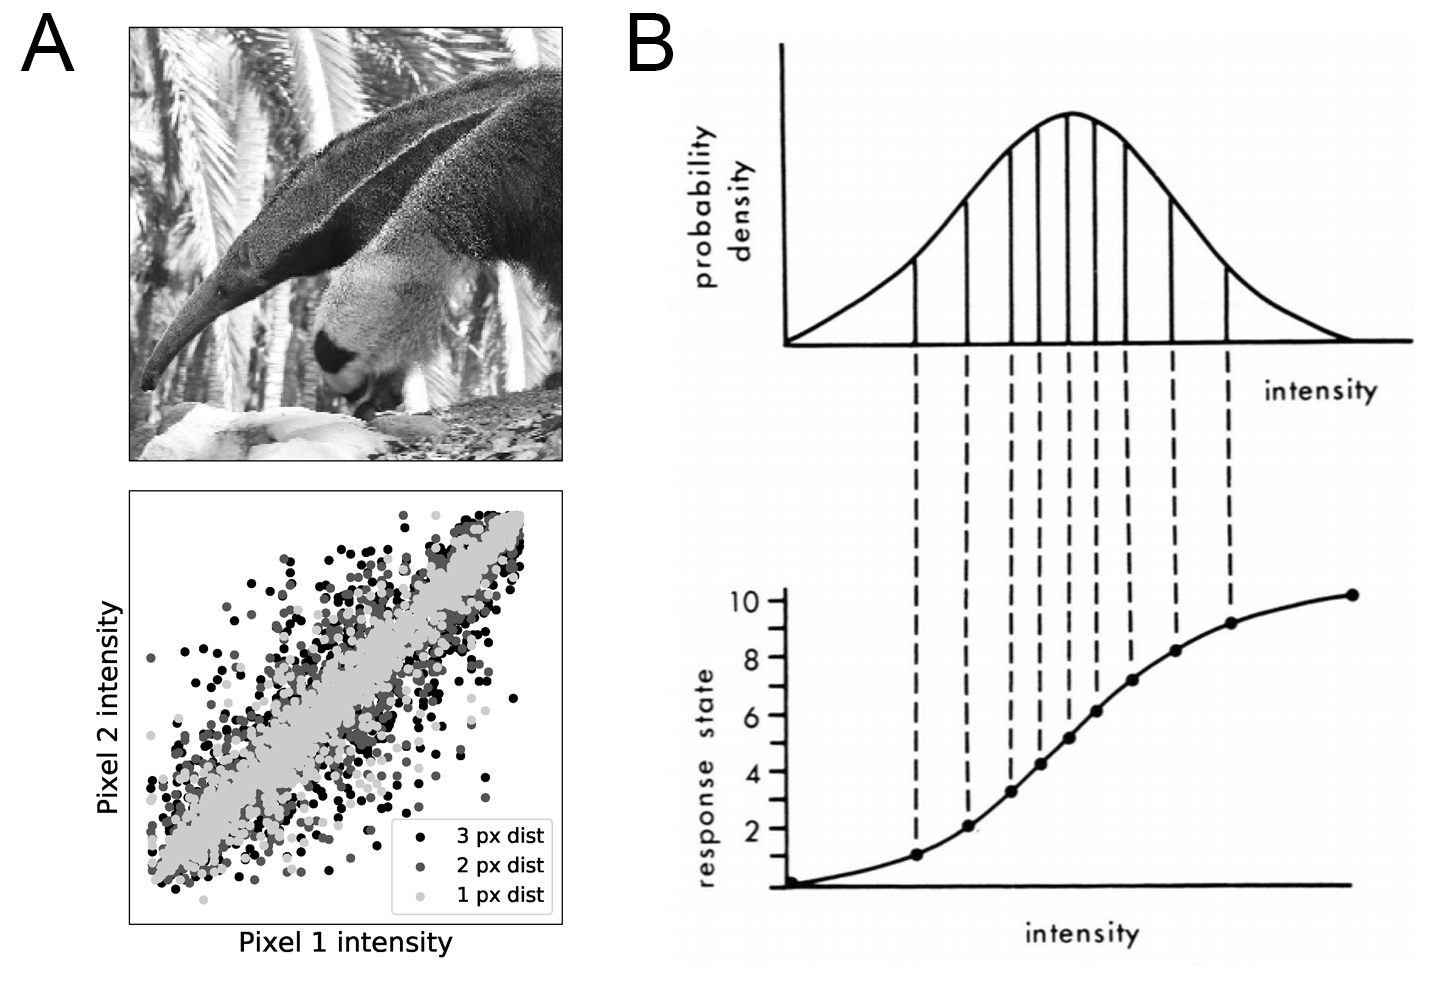
\includegraphics[width=\textwidth]{fig-rev2-ech}
    \caption{Efficient coding hypothesis.
    \textbf{\emph{A}},
         Sensory stimuli in the environment, such as an image of \revise{an anteater},
         display significant statistical structure. For example, the luminance
         value of nearby pixels in the image are significantly correlated,
         an effect that exists even for nonadjacent pixels \revise{(inspired by \cite{LouieGlimcher2012})}.
         Neural systems can improve their coding efficiency by accounting
         for and reducing such information redundancy.
     \textbf{\emph{B}},
         For a given distribution of sensory characteristics in the world \revise{(top)},
         \revise{a neuron's information capacity is maximized 
         when all response levels are used with equal frequency
         (reprinted from \cite{Laughlin1981} under CC-NC-ND 3.0).
         Intervals between each response level encompasses an equal area
         under the intensity distribution, so each state is used with
         equal frequency.}
    }
	\label{fig:ech}
\end{figure}


Extending this idea to the neural level,
Barlow \cite{Barlow1961} proposed that
the goal of early neurons in sensory processing is to remove
the redundancy in the input stimuli.
These ideas were shaped by two
fundamental empirical observations
about early visual cortex:
1) a neuron's \ac{RF} resembled a decomposition of the visual
stimulus into a series of local, largely independent feature components
(e.g., a 2-D Gabor function is basically a local approximation of the
directional spatial derivative of an image),
and 2) any individual neuron responded only sparsely to a small subset of
stimulus features (e.g., orientation or color at a particular spatial location).
Thus a neuron's \ac{RF} could be understood as a
sparse, low-dimensional embedding of high-dimensional input stimuli
\cite{Barbieri2015}.
\revise{However, there is the possibility that sparsity results from a limited stimulus set as we discuss in the ``Model limitations'' section.}

At the level of single neurons, efficient coding requires
that a neuron's input-output function be adjusted so that all
activity levels are used equally in response to a specific
stimulus distribution \cite{Simoncelli2003} (see Fig.~\ref{fig:ech}B).
If the input-output function sensitivity is too low,
high levels of the stimulus feature will be indistinguishable
as the response function saturates; if the sensitivity is set too high,
low levels of the stimulus feature cannot drive responses 
\cite{Laughlin1981}.

At the level of neuronal populations,
neural responses should be both \emph{decorrelated}
(i.e., independent from one another)
and \emph{sparse}
(i.e., involve only a small fraction of neurons in the population)
\cite{LouieGlimcher2012}.


\subsection*{Sparse coding}

Taking these ideas a step further,
Olshausen and Field \cite{OlshausenField1996b} 
noted that natural images contain statistical
dependencies beyond linear pairwise correlations among image pixels,
and argued that these higher-order correlations should be taken into
account when developing an efficient code.
Their goal was thus to find a linear coding strategy
capable of reducing these higher-order forms of redundancy.

\emph{Linear sparse coding} is one such strategy,
where monochromatic images $I(x,y)$
are described in terms of a linear superposition of
a number of \textbf{basis functions},
$w_b(x,y)$:
\begin{equation}
I(x,y) = \sum^B_{b=1} w_b(x,y) h_b,
\label{eqn:sparse-coding}
\end{equation}
where $h_b$ are stochastic coefficients that are different for each image
\cite{OlshausenField1996,Hyvarinen2001}.
Learning a sparse code for images thus involved determining
the values of both $w_b(x,y)$ and $h_b$ for all $b$ and $(x,y)$,
given a sufficient number of observation of images,
under the constraint that $h_b$ be sparse.
In this context, $h_b$ was considered sparse if it took very small
or very large (absolute) values more often than a Gaussian random
variable would \cite{Hyvarinen2001}.
This sparsity constraint allowed for basis functions that were not
needed to describe a given image structure to be weeded out.

\revise{Sparsity, in this context, is an information-theoretic concept
related to how efficiently and completely information is encoded with
the basis functions described above.
Please note that this is different from empirical observations
of brain areas being `sparsely' activated; that is,
sparse population activity does not necessarily imply that a brain area
implements a sparse coding scheme.
This confusion is fueled in part by the wide variety of definitions of sparsity
used in the literature\cite{SpanneJorntell2015,BarthPoulet2012}.}

When Olshausen and Field applied linear sparse coding 
to natural images,
they found that the emerging basis functions 
were qualitatively similar in form
to \acp{RF} of simple cells in \ac{V1} 
\cite{OlshausenField1996,OlshausenField1997},
thus giving empirically observed \acp{RF} 
an information-theoretic explanation.
In this context, $h_b$ in Eq.~\ref{eqn:sparse-coding} above
corresponded to the (signed) activation value of a particular \ac{V1}
neuron, and $w_b(x,y)$ were the connection weights
(or \emph{synaptic weights} in an artificial neural network)
that were closely related to that neuron's \ac{RF}.
Olshausen and Field went on to show that 
the set of basis functions that best described \ac{V1} \acp{RF} 
was greater in number than the effective
dimensionality of the input
(\revise{which they termed} an \emph{overcomplete} basis set) 
\cite{OlshausenField1997}.
\revise{It is worth noting that sparse coding with an overcomplete basis set
is typically associated with an anatomical fan-out motif,
such as expanding 1 million optic nerve fibers 
into more than 100 million \ac{V1} neurons,
or from a small number of mossy fibers to a 100-fold larger number of
granule cells in the cerebellum.}

However, as pointed out by Hoyer \cite{Hoyer2003}, 
linear sparse coding falls short of providing a literal interpretation
for \ac{V1} simple-cell behavior for two reasons:
1) every neuron could be either positively or negatively active, and
2) the input to the neural network was typically double-signed,
whereas \ac{V1} neurons receive visual input from the \ac{LGN} 
in the form of separated, nonnegative ON and OFF channels.

In order to transform Olshausen and Field's sparse coding
from a relatively abstract model of image representation 
into a biologically plausible model of early visual cortex processing,
Hoyer \cite{Hoyer2002,Hoyer2003} thus proposed to enforce
both input signal and neuronal activation to be nonnegative.
This seemingly simple change had remarkable consequences 
on the quality of the sensory representation:
Whereas elementary image features in the standard sparse coding model
could `cancel each other out' through subtractive interactions,
enforcing nonnegativity ensured that features combined additively,
much like the intuitive notion of combining parts to form a whole.
The resulting parts-based representations resembled \acp{RF} in \ac{V1} 
much more closely than other holistic representations.
These considerations led to the formulation of nonnegative sparse coding (\ac{NSC}) in its current form.


\subsection*{Nonnegative sparse coding (NSC)}

As a special case of linear sparse coding,
\ac{NSC} shares the same goal of accurately describing observed data
as a superposition of a set of sparsely activated basis functions.
However, \ac{NSC} additionally requires 
all basis functions and activation values
(i.e., $w_b(x,y)$ and $h_b$ in Eq.~\ref{eqn:sparse-coding})
to be nonnegative.

Consider $S$ observed stimuli or data samples,
each comprised of $F$ observed feature values,
such as a collection of $S$ images $I(x,y)_s$ ($s \in [1, \ldots, S]$)
from the example above,
each consisting of $F$ different grayscale values.
If we arrange the observed feature values of the $s$-th observation into
a vector $\vec{v}_s$ (i.e., by flattening each observed image),
and if we arrange all vectors into the columns 
of a $F \times S$ data matrix \textbf{V},
then linear decompositions describe these data as:
\begin{equation}
\mathbf{V} \approx \mathbf{WH},
\label{eqn:linear-decomposition}
\end{equation}
where \textbf{W} is a $F \times B$ matrix that contains as its columns
the $B$ basis functions of the decomposition
(i.e., the $b$-th column of \textbf{W} corresponding to 
$w_b(x,y)$ $\forall x,y$ in Eq.~\ref{eqn:sparse-coding}),
and \textbf{H} is a $B \times S$ matrix containing
as its columns the activation values 
of each basis function for a particular input stimulus
(i.e., the $b$-th column of \textbf{H} corresponding to 
$h_b$ $\forall b$ in Eq.~\ref{eqn:sparse-coding}).
The difference between \textbf{V} and \textbf{WH} is termed
the \emph{reconstruction error}.

The goal of \ac{NSC} is then to find a linear decomposition of \textbf{V}
that minimizes the reconstruction error,
while guaranteeing that \textbf{H} is sparse.
This can be achieved by minimizing the following cost function
\cite{Hoyer2002}:
\begin{equation}
\min_{\mathbf{W}, \mathbf{H}} \frac{1}{2} ||\mathbf{V} -\mathbf{WH}||^2 + \lambda \sum_{ij} f(\mathbf{H}_{ij}),
\label{eqn:nsc-cost-function}
\end{equation}
subject to the constraints
$\forall ij: \mathbf{W}_{ij} \geq 0$, $\mathbf{H}_{ij} \geq 0$, and
$||\vec{w}_i|| = 1$, where $\vec{w}_i$ denotes the 
$i$-th column of \textbf{W}.
Here, the left-hand term describes the reconstruction error,
whereas the right-hand term describes the sparsity of the decomposition.
The trade-off between accurate reconstruction and sparsity
is controlled by the parameter $\lambda$ ($\lambda \geq 0$), whereas
the form of $f$ defines how sparsity is measured
(a typical choice is the L1 norm on \textbf{H}).
\revise{\Ac{NSC} explicitly discourages statistically inefficient representations,
because strongly accounting for a rare observation 
at the expense of ignoring a more common one stimulus component
would result in an increased reconstruction error.}

In the case of $\lambda = 0$, Eq.~\ref{eqn:nsc-cost-function}
reduces to the squared-error version of \textbf{\ac{NMF}}.
Although \ac{NMF} enforces all elements of \textbf{W} and \textbf{H}
to be nonnegative,
the resulting decomposition might not be sparse,
depending on the number of basis functions $B$.
In order to emphasize decompositions where \textbf{H} is sparse,
Eq.~\ref{eqn:nsc-cost-function} should be minimized 
with $\lambda > 0$ \cite{Hoyer2002}.

Another open parameter is the number of basis functions, $B$, 
which controls the predictive power of the model,
and must be determined empirically.
With a small number of basis functions,
\ac{NSC} is unlikely to achieve a low reconstruction error
be it in familiar contexts (training data) or in novel contexts
(held-out test data).
In this case, the error depends on the systematic bias of the model,
and the model is said to \emph{underfit} the data
(left-hand side of Fig.~\ref{fig:nsc-bias-variance-dilemma}).
With increased model complexity,
the model can learn subtle differences 
between different contexts with high accuracy,
leading to a reduced bias (training) error.
However, with increased complexity, the model is more likely to learn
patterns between training contexts that arise either from underlying noise
or from spurious correlations. As a result,
the model will respond according to
these learned patterns when a novel context is presented
(rather than according to the underlying actual relationships), 
in which case the model is said to \emph{overfit} the data
(right-hand side of Fig.~\ref{fig:nsc-bias-variance-dilemma}).
Hence, the goal of a successful model is to find the ideal compromise
in the bias-variance error trade-off \cite{Beyeler2017}
(labeled `best model' in Fig.~\ref{fig:nsc-bias-variance-dilemma}).

\begin{figure}[h]
	\centering
% 	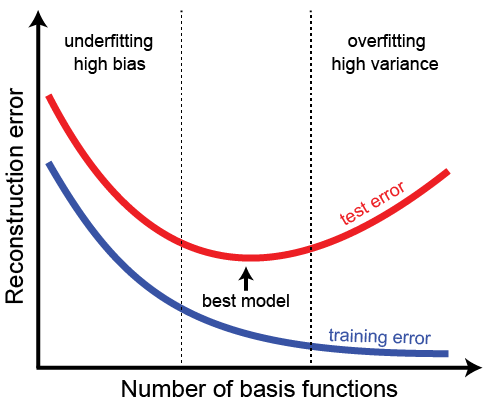
\includegraphics[width=0.6\textwidth]{fig-rev1-bias-variance}
    \caption{The bias-variance dilemma.
    With increased model complexity 
    (i.e., with an increased number of basis functions), 
    the reconstruction error on a set
    of familiar (training) data typically decreases until it reaches zero.
    In contrast, the reconstruction error on a set of unfamiliar, held-out
    (test) data typically goes through a minimum as a function of model complexity.
    A successful model chooses the number of basis functions such that the
    generalization (test) error is minimized (labeled `best model`).}
	\label{fig:nsc-bias-variance-dilemma}
\end{figure}

Analogously to \cite{OlshausenField1996,OlshausenField1997},
the basis functions obtained in \ac{NSC} can be interpreted as
the connection weights of a population of simulated neurons
in an artificial neural network.
In other words, under \ac{NSC} the number of basis functions $B$ 
corresponds to the number of output neurons, and the
response of the $b$-th model output neuron
($b \in [1, ..., B]$)
to a particular input stimulus $s$, termed $r_{bs}$,
can be computed by feeding the dot product of
that neuron's connection weights
(i.e., the $b$-th column in $\mathbf{W}$, $\vec{w}_b$)
and a data vector
(i.e., the $s$-th column in \textbf{V}, $\vec{v}_s$)
to an activation function $\Theta$:
\begin{equation}
r_{bs} = \Theta(\vec{w}_b \cdot \vec{v}_s),
\label{eqn:nsc-model-response}
\end{equation}
where $\cdot$ denotes the dot product.
For example, the linear response of a model neuron
can be calculated by setting $\Theta$ to the identity function $\Theta(x)=x$.
Note that the response of the model neuron to different stimuli 
$s \in [1, \ldots, S]$
involves different columns of \textbf{V},
but always relies on $\vec{w}_b$.

Inhibitory connections can be modeled in the same fashion,
by interpreting inhibitory connection weights
as nonnegative synaptic conductances.
\revise{For example, Hoyer \cite{Hoyer2003} used \ac{NSC} to model \ac{V1} neurons
as receiving input from both excitatory ON and inhibitory OFF cells in the \ac{LGN}.
Using pre-whitened natural images, Hoyer sampled $12 \times 12$ pixel patches from
the images, and then separated positive and negative values into separate channels.
Each image patch was thus represented by a $2 \times 12 \times 12 = 288$ dimensional vector,
each element of which mimicked the activity of an ON or OFF cell
in response to the image patch.
These vectors were then arranged into the columns of \textbf{V}.}
This procedure not only preserved the parts-based quality of the encoding,
but also allowed for more complicated connection types to be modeled.
However, it is interesting to note that a more recent study has argued
that the nonnegativity constraint on the
connection weights might not be necessary 
to preserve the parts-based quality of the encoding (see \cite{Liu2017}).

Thus, we can utilize \textbf{W} 
(which must remain fixed once learned)
and Eq.~\ref{eqn:nsc-model-response}
to simulate a model neuron's response to arbitrary input stimuli
by replacing the column in \textbf{V} with new input.
This allows us to investigate the response properties 
of individual model neurons
much in the same way that experimental neuroscientists 
study biological neurons.
This is important because it means that \ac{NSC} can be used to 
model neural activity in the brain, 
and the resulting activity patterns generated by \ac{NSC}
can be compared to and evaluated against experimental findings. 


\section*{Empirical evidence for nonnegative sparse coding in the brain}

An influential paper by Lee and Seung \cite{LeeSeung1999}
found that applying \ac{NMF} to a database of face images
yielded sparse, localized features that resembled parts of a face
\revise{(Fig.~\ref{fig:NMF|reconstruction}A)}.
In their case, \ac{NMF} acted on a
$F \times S$ data matrix \textbf{V},
whose rows corresponded to distinct features of the input 
(e.g., $F$ different pixels of an image)
and whose columns corresponded to different stimuli or 
observations of those features
(e.g., $S$ different images).
\ac{NMF} was used to decompose the matrix into two reduced-rank matrices
(Fig.~\ref{fig:NMF|reconstruction}, \revise{inset})
whose linear combination could be weighted such that the product of \textbf{W} and \textbf{H} provided an accurate reconstruction of \textbf{V}
\revise{(see Eq.~\ref{eqn:linear-decomposition}).}

A particular image, in this case encoded by $F = 19 \times 19 = 361$ pixels
could be accurately represented by a linear combination of 
a small number ($B = 49$) of encoding variables or `basis images'
(Fig.~\ref{fig:NMF|reconstruction}\revise{A}).
Such a representation is reminiscent to neural processing in \ac{IT},
an area in the ventral visual `what' stream
involved in encoding high-level object identity
\cite{BrincatConnor2004,Majaj2015},
where images of whole faces can be linearly reconstructed
using responses of approximately $200$ neurons
that each respond to a certain set of physical facial features
\cite{ChangTsao2017}.

\begin{figure}[ht]
	\centering
% 	\includegraphics[width=\textwidth]{fig4}
    \caption{\revise{Sparse and parts-based representations recovered by \ac{NMF}
             resemble receptive fields across brain regions.
             \Ac{NMF} (inset) can reconstruct a} data matrix \textbf{V}
             ($F$ features x $S$ stimuli)
             from two reduced-rank matrices \textbf{W}
             (containing $B$ basis functions) and \textbf{H}
             (containing the hidden coefficients of the decomposition).
             Any individual input stimulus (i.e., column in \textbf{V}, \revise{red})
             can be reconstructed from a linear combination
             \revise{(i.e., column in \textbf{H}, blue)}
             of a set of basis functions (i.e., all columns in \textbf{W}, 
             \revise{green}).
         \textbf{\emph{A}},
             A facial image can be reconstructed from a sparse activation
             of simulated \acs{IT} neurons that
             preferentially respond to parts of faces
             (adapted from \cite{LeeSeung1999}).
         \textbf{\emph{B}},
             An optic flow field can be reconstructed from a sparse
             activation of model \acs{MSTd} neurons that prefer various
             directions of 3D self-translation and self-rotation
             (adapted from \cite{Beyeler2016}).
         \textbf{\emph{C}},
             A rat's 2D allocentric position and route-based direction of
             motion can be reconstructed from a sparse activation of
             model \acs{RSC} neurons that prefer an intricate combination of
             linear velocity (LV), angular velocity (AV), head direction (HD)
             and 2D position (P).
             For the sake of clarity, only the 4 most contributing hidden
             coefficients (out of 30) are shown.}
	\label{fig:NMF|reconstruction}
\end{figure}


\revise{Interestingly}, such a parts-based representation is not specific to
information processing in \ac{IT};
the same principle can be extended to other areas of the visual system,
such as the \ac{MSTd},
which is part of the visual motion pathway \cite{Beyeler2016}.
Neurons in \ac{MSTd} respond to relatively large and complex patterns
of retinal motion (`optic flow'),
owing to input from direction and speed selective neurons in the \ac{MT}
(for a recent review, see \cite{Orban2007}).
Although \ac{MSTd} had long been suspected to be involved in the
analysis of self-motion,
the complexity of neuronal response properties has made it difficult
to experimentally investigate how neurons in \ac{MSTd}
might perform this function.
However, when \revise{our group} 
applied \ac{NMF} to 
\revise{simulated neural activity patterns whose statistical properties
resembled that of experimentally recorded \ac{MT} neurons} 
\cite{Beyeler2016},
\revise{we} found a sparse, parts-based representation of retinal flow
(Fig.~\ref{fig:NMF|reconstruction}\revise{B})
similar to the parts-based representation of faces
encountered by Lee and Seung \cite{LeeSeung1999}.
The resulting `basis flow fields' showed a remarkable resemblance to receptive fields
of \ac{MSTd} neurons, as they \revise{responded to}
an intricate mixture of
3D translational and rotational flow components
in a subset of the visual field.
As a result, any flow field possibly to be encountered 
during self-movement through a 3D environment
could be represented by only $B = 64$ simulated \ac{MSTd} neurons,
as compared to $F = 9,000$ simulated \ac{MT} input neurons.
This led to an sparse \revise{and parts-based} population code,
where any given stimulus could be represented
by only a small number of simulated \ac{MSTd} neurons
\cite{Beyeler2016}.

Analogously, \ac{NSC} can explain response properties
of neurons outside the visual system, 
such as in the \ac{RSC}, an area in the posterior cingulate region
important for navigation and spatial memory \cite{Miller2014,Nelson2015,VannAggleton2009}.
Neurons in the \ac{RSC} conjunctively encode multiple variables related to the environment and one's position and movement within it
\revise{(e.g., position, head direction, linear velocity, and angular velocity)},
allowing the representation of spatial features of the environment 
with respect to multiple reference frames \cite{AlexanderNitz2015}.
\revise{When our group applied \ac{NMF} to neurophysiological data from
\ac{RSC} neurons while rats ran back and forth on a W-shaped track
(for experimental details, see Supplementary Materials),
we again found a sparse and parts-based representation for behaviorally
relevant variables such as the animal's position, head direction, 
and movement direction (Fig.~\ref{fig:NMF|reconstruction}C).
Interestingly, model \ac{RSC} neurons encoded these variables with respect
to multiple frames of reference
(e.g., head direction: \textbf{allocentric reference frame},
linear velocity: \textbf{route-based reference frame}).
Once again, the dimensionality of the stimulus space was drastically reduced
from $F = 417$ input neurons to a set of $B = 30$ model \ac{RSC} neurons.}

\revise{Due to its roots in efficient-coding theories of natural image processing,
there is a large body of research highlighting the role of \ac{NSC} in
visual cortex function
(e.g., \cite{Barlow1961,OlshausenField1996,Hoyer2003,BenHamed2003}).}
Although there seems to be a consensus that 
information-theoretic explanations are relevant 
when investigating the early visual system,
higher-order brain areas are often considered to be specialized for
performing tasks
(e.g., recognizing objects, making decisions, navigating an environment),
rather than the efficient encoding of information.

\revise{However, more recently, 
\ac{NSC}-like computational models have found application outside visual cortex,
where they have started to provide compelling evidence that a wide variety of
neuronal response properties can be understood as an epiphenomenon
of efficient population coding based on dimensionality reduction.
Examples include elucidating the dimensions along which perceptual space
is organized in the olfactory system
\cite{MorenoBoteDrugowitsch2015,Castro2013},
the coordination of movement in the cortico-basal ganglia-thalamo-cortical loop
\cite{BarGad2000,BarGad2003_Review},
and the combined representation of allocentric and route-based 
spatial navigation cues
in retrosplenial cortex \cite{Rounds2018}.}
\revise{The success of these models suggests that \ac{NSC}}
might apply elsewhere in the brain, 
\revise{thus warranting further investigation.}
In fact, sparse (and potentially parts-based) representations have been observed
in \revise{a wide variety of brain areas}
(see Table~\ref{table:listEvidence}).
This introduces the \revise{intriguing} possibility that \ac{NSC} might
be a general principle to which \revise{many} neuronal computations adhere.
\revise{In the future, \ac{NSC} might provide a useful theoretical framework
under which to understand the often complex and nonintuitive response properties
of neurons in brain areas far removed from sensory inputs,
including the selection and integration of various task-related variables
in prefrontal cortex
\cite{Mante2013}
and the ability of premotor cortex to prepare movements without executing them
\cite{Kaufman2014}.}



\begin{table}[ht]
\begin{adjustwidth}{-2.25in}{0in}
	\centering
	\caption{Nonnegative sparse coding in the brain.
    We list a group of brain regions for which there is experimental evidence of certain features associated with NSC (`X': evidence exists, `?': has yet to be investigated).
   For each brain region, the left-hand side of the table lists experimental evidence for sparse \revise{population codes} and/or parts-based representations, whereas the right-hand side lists computational support that \revise{\ac{NSC}-like models} can describe receptive fields or response properties within that region.}
    \def\arraystretch{1.1}
    {\setlength{\tabcolsep}{1em}
    \begin{tabular}{r|rrr|rr}
	\revise{\textbf{Brain}} & \textbf{Sparse} &  \textbf{Parts-} & \textbf{Experimental} & \textbf{Modeled} & \textbf{Computational} \\
	\textbf{Area} & \revise{\textbf{code}} & \textbf{based} & \textbf{evidence} & \textbf{by NSC} & \textbf{ support} \\ \hline
    Retina & X & X & \cite{Onken2016,Liu2017} & X & \cite{Onken2016,Liu2017} \\
    \revise{Visual cortex} & X & X & \pbox{5cm}{\cite{OlshausenField1996,HoyerHyvarinen2002,vanHateren1998,Wachsmuth1994,FreiwaldTsao2010,ChangTsao2017,BenHamed2003}} & X & \pbox{5cm}{\cite{OlshausenField1996,Hoyer2003,Carlson2013,Hyvarinen2001,LeeSeung1999,Hosoda2009,Beyeler2016}} \\
    Auditory cortex & X & \revise{X} & \revise{\cite{Hromadka2008,rokem2006,bendor2008,Leaver2010,Terashima2013,SmithLewicki2006}} & \revise{X} & \revise{\cite{Martinez2015,David2007}} \\
 	Olfactory cortex & X & \revise{X} & \cite{Koulakov2011,poo2009,rinberg2006,Broome2006,Castro2013} & \revise{X} & \revise{\cite{MorenoBoteDrugowitsch2015,Castro2013}}  \\
 	\revise{Somatosensory} cortex & X  & \revise{X} & 			   \revise{\cite{Jadhav2009,oconnor2010,Crochet2011,Ramirez2014,penfield1937,hari1993,petersen2007}} & \revise{X} & \revise{\cite{WhitewayButts2017,Hafner2004}}  \\
    \revise{Parietal cortex} & \revise{?} & \revise{X} & \revise{\cite{Poggio1990,PougetSejnowski1997,andersen1997multimodal,PougetSnyder2000,louie2015adaptive}} & \revise{?} & \revise{?}  \\
    Retrosplenial cortex & \revise{?} & X & \revise{\cite{AlexanderNitz2015,vedder2016,mao2017}} & X & \cite{Rounds2018} \\
    \revise{Prefrontal cortex} & \revise{?} & \revise{?} & \revise{\cite{Mante2013,Rigotti2013,Fujisawa2008,Wei2015}} & \revise{?} & \revise{?}  \\    
    Motor cortex & \revise{?} & \revise{?} & \revise{\cite{Beloozerova2003,penfield1937,GrazianoAflalo2007,Brecht2004}}
    & ? & \revise{?} \\
    Hippocampus & \revise{X} & \revise{?} & \revise{\cite{ThompsonBest1989,Bakker2008,myers2011pattern,rolls2013,Wixted2014,Poli2017}} & \revise{?} & \revise{?} \\        
    Basal ganglia & X & ? & \cite{BarGad2003_Review,Turner2000,schwab2015} & X & \pbox{5cm}{\cite{BarGad2000,BarGad2003_Review}} \\  
	\end{tabular}}
    \label{table:listEvidence}
\end{adjustwidth}
\end{table}

\revise{In the following subsections,
we review existing experimental evidence
for sparse and parts-based representations 
in various brain areas highlighted in Table~\ref{table:listEvidence}.
Where available, we highlight \ac{NSC}-like computational models
that  successfully explain response properties of individual neurons
or have been instrumental in elucidating the dynamics at the population level.}


\subsection*{NSC in the retina and visual cortex}

Due to its roots in efficient-coding theories of natural image processing,
\ac{NSC} figures prominently in the vision neuroscience literature.

For example, \ac{NMF}-based models were able to reconstruct
\emph{in vitro} neuronal spike trains from the salamander retina 
\cite{Onken2016,Liu2017}.
By combining spike-triggered average with \ac{NMF},
Liu and colleagues \cite{Liu2017} were able to identify the subunit layout
of retinal ganglion cells
(Fig.~\ref{fig:NMF|retina}).
Whereas modules were constrained to have nonnegative elements,
stimuli were represented by their contrast values (i.e., their relative deviation from mean light intensity, which could be positive or negative).
The goal of their \ac{NMF} variant was then to seek weights and nonnegative modules
that minimize the difference, in a least-squares sense, between the spike-triggered
stimuli and the reconstruction.
Interestingly, the identified subunits corresponded to 
individual presynaptic bipolar cells,
as verified by multielectrode array recordings with simultaneous recordings from
individual bipolar cells through sharp microelectrodes \cite{Liu2017}.
This allowed the researchers to improve predictions about how ganglion cells respond
to natural stimuli, without the need to guess a specific model structure that may be constrained in terms of the size, shape, number, or nonlinearity of 
ganglion cell subunits.
\mikeNote{R1: Fig.5, provide a succinct summary or schematic of STNMF. Also, panel A is not very clear to me (although I haven’t looked at the source paper). Panel B: are the subunits and the modules the same?}

\begin{figure}[ht]
	\centering
	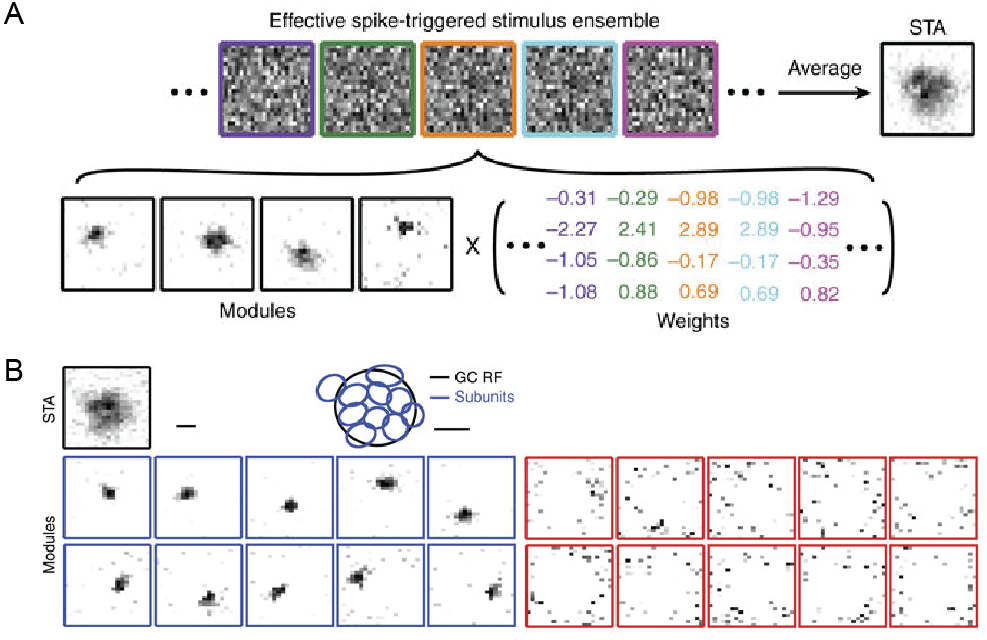
\includegraphics[width=\textwidth]{fig-rev1-retina}
    \caption{
    Identification of retinal ganglion cell subunits 
    with \ac{STNMF} (adapted from \cite{Liu2017}).
    \textbf{\emph{A}},
	     Samples of a ganglion cell’s effective spike-triggered stimulus ensemble (top),
         whose average corresponds to the cell’s \ac{STA}.
         For easier visual comparison with the subunits,
         \acp{STA} are displayed with negative pixel values set to zero and
         with zero corresponding to white in the grayscale image.
         \ac{STNMF} decomposes this ensemble into a set of modules and 
         a weight matrix (bottom).
         The example here shows four modules that were identified for
         a sample ganglion cell.
    \textbf{\emph{B}},
         Modules obtained for another sample ganglion cell by applying \ac{STNMF}
         with 20 modules (bottom 2 rows). Some modules have a strongly localized structure 
         (blue frames), others are more noise-like (red frames).
         The top row shows the cell’s receptive field,
         given by the spatial component of the STA, as well as the fitted \ac{RF} outline
         (GC RF, black ellipse), together with outlines of the localized subunits 
         (blue ellipses). Scale bars, 100 µm.
    }
	\label{fig:NMF|retina}
\end{figure}

As mentioned in the previous section,
\ac{NSC} has been extensively applied to early visual cortex,
where it has successfully explained 
orientation and frequency tuning of simple and complex cells in \ac{V1} \cite{Hoyer2003},
edge-like pooling of spatial frequency channels in V2 \cite{Hyvarinen2005},
including \ac{RF} properties such as end-stopping and contour integration 
\cite{HoyerHyvarinen2002}.
With the exception of face processing in \ac{IT}
\cite{LeeSeung1999,ChangTsao2017},
\ac{NSC} has yet to be applied to higher-order areas in the ventral visual stream.
The success of \ac{NSC} in explaining V1 and V2 response properties
suggests that it might be possible to extend the model to texture integration in
V4.

In our own work, we found evidence for \ac{NSC} in the dorsal visual stream.
Specifically, we demonstrated that simulated neurons 
in a \ac{NSC} based model of \ac{MSTd} 
responded to  large optic flow fields in much the same way as real neurons in macaque \ac{MSTd} \cite{Beyeler2016}.
Fig.~\ref{fig:NMF|MSTd} shows the distribution of direction preferences
of \ac{MSTd} cells (Fig.~\ref{fig:NMF|MSTd}A, B; \cite{Takahashi2007})
and \ac{MSTd}-like model units (Fig.~\ref{fig:NMF|MSTd}C, D; \cite{Beyeler2016})
for \revise{rotation and translation, respectively}.
Each data point in the scatter plots specifies the preferred 3D direction
of a single neuron or model unit.
Histograms along the boundaries show the marginal distributions of azimuth
and elevation preferences.
Not only did individual units match response properties of individual neurons
in macaque \ac{MSTd},
but the model was able to recover statistical properties of the \ac{MSTd}
population as a whole, such as a relative overrepresentation of lateral
headings (Fig.~\ref{fig:NMF|MSTd}C, D).

\begin{figure}[ht]
	\centering
	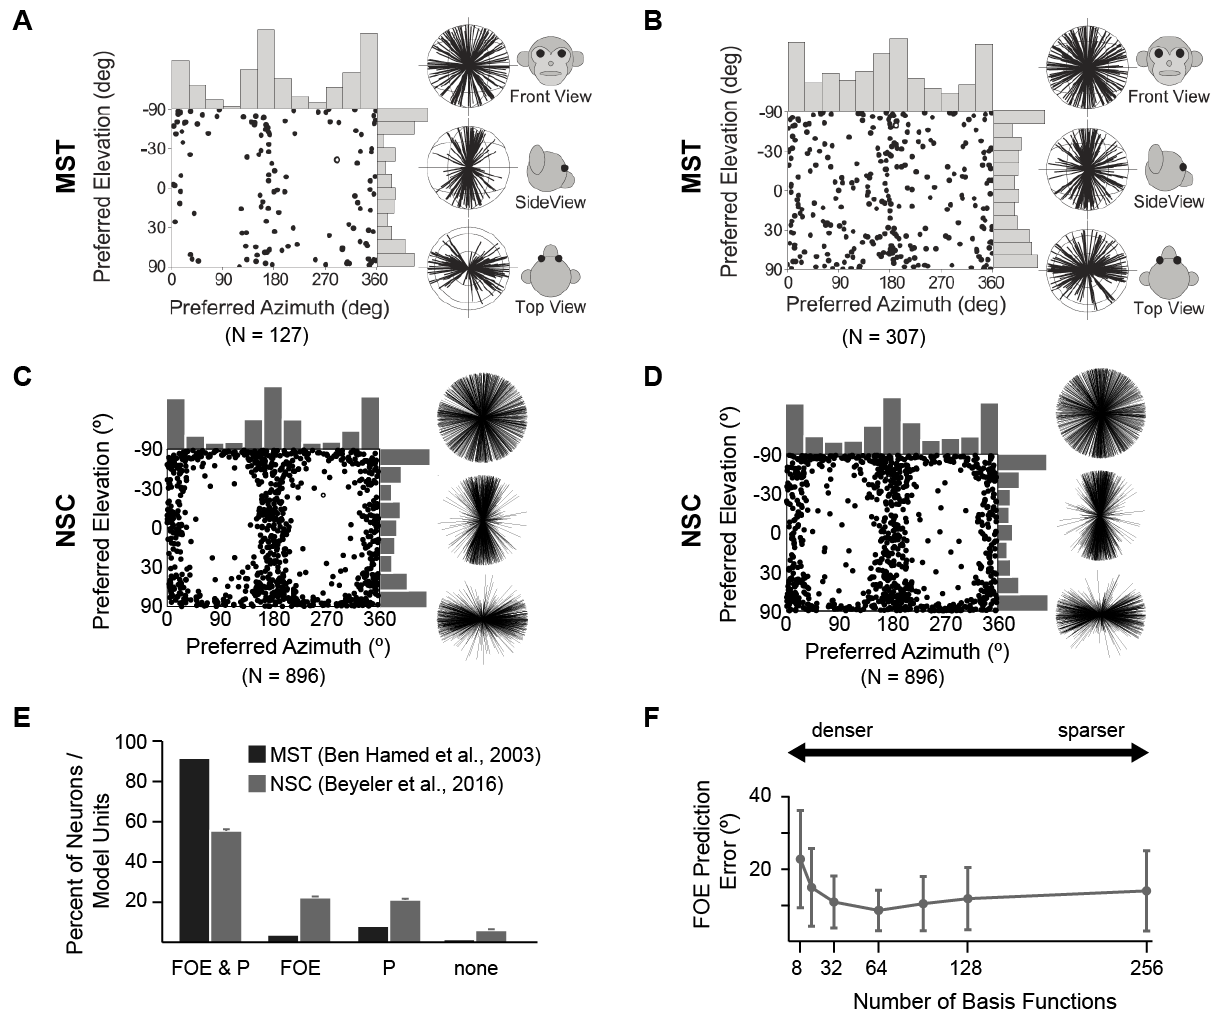
\includegraphics[width=0.97\textwidth]{fig-rev1-MST}
    \caption{
    \textbf{\emph{A-D}},
         Distribution of 3D direction preferences of macaque \ac{MSTd} neurons
         (rotation, \textbf{\emph{A}}; translation, \textbf{\emph{B}}; 
         reprinted from \cite{Takahashi2007})
         and model units in the \ac{NSC}-based sparse decomposition model
         (rotation, \textbf{\emph{C}}; translation, \textbf{\emph{D}}; 
         reprinted from \cite{Beyeler2016}).
         Each data point in the scatter plots corresponds to the preferred azimuth
         (abscissa) and elevation (ordinate) of a single neuron.
         Histograms along the top and right sides of each scatter plot show the
         marginal distributions.
         Also shown are 2D projections (front view, side view, and top view)
         of unit-length 3D preferred direction vectors (each radial line represents
         one neuron).
    \textbf{\emph{E}},
         Distribution of focus of expansion (FOE) and pursuit (P) selectivities
         in macaque \ac{MSTd} (dark gray) and model \ac{MSTd} (light gray;
         reprinted from \cite{Beyeler2016}).
         Neurons or model units were involved in encoding heading (FOE),
         eye velocity (P), both (FOE \& P), or neither (none).
    \textbf{\emph{F}},
         Heading prediction (generalization) error as a function of the
         number of basis functions using 10-fold cross-validation.
         Vertical bars are the SD (reprinted from \cite{Beyeler2016}).
    }
	\label{fig:NMF|MSTd}
\end{figure}

\ac{MSTd} is known to encode a number of perceptual variables,
such as the direction of travel (heading) and eye rotation velocity.
During forward movement, retinal flow radiates out symmetrically from a single point,
the focus of expansion (FOE), from which heading can be inferred.
However, instead of consisting of a set of distinct subpopulations,
each specialized to encode a particular perceptual variable,
\ac{MSTd} has been found to consist of neurons that act more like basis functions,
where a majority of cells were involved in the simultaneous encoding of multiple
perceptual variables (Fig.~\ref{fig:NMF|MSTd}E).
A similar picture emerged when we investigated the involvement of \ac{MSTd}-like
model units in the encoding of both heading and eye rotation velocity
(Fig.~\ref{fig:NMF|MSTd}E).

Interestingly, the sparsity regime in which model \ac{MSTd} achieved the
lowest heading prediction error (Fig.~\ref{fig:NMF|MSTd}F) was also the
regime in which \ac{MSTd}-like model units reproduced a variety of known
\ac{MSTd} visual response properties
(for experimental details refer to \cite{Beyeler2016}).
In contrast to findings about early visual cortex,
this regime does not use an overcomplete basis set \cite{OlshausenField1996},
yet can still be considered a sparse coding regime \cite{SpanneJorntell2015}.
Such an intermediary sparse code might be better suited
(as opposed to an overcomplete basis set)
for areas such as \ac{MSTd},
because the increased memory capacity of such a code might lead to compact
and multifaceted encodings of various perceptual variables
\cite{BenHamed2003}.


\subsection*{NSC in the auditory cortex}

The auditory cortex is a prime example of efficient coding. The auditory system is believed to decompose auditory signals into
a set of elementary acoustic features \cite{SmithLewicki2006},
such that the complete acoustic waveform can be described by a
sparse population code that operates near an information-theoretic optimum
\cite{SmithLewicki2006,rokem2006,Hromadka2008}.
It is therefore not surprising that computational models based on \ac{NSC}
have been very successful at describing the spectro-temporal \acp{RF}
of neurons in the \ac{A1} \cite{Martinez2015,David2007}.
Response properties of \ac{A1} neurons are well described by a spectrogram;
they are often tuned to stimulus frequency but are rarely phase-locked
to oscillations of the sound waveform \cite{Leaver2010}.
The cortical representation of auditory signals seems to not only be sparse,
but also rely on statistically independent acoustic features \cite{Klein2003}.

Similar to visual cortex, auditory cortex is hierarchically organized,
with neurons in \ac{A1} responding to simple acoustic features of natural sounds,
and higher-order areas responding to more behaviorally relevant stimuli.
The anterior superior temporal region of auditory cortex, for example,
responds to categories of acoustic objects,
such as sounds produced by voices and musical instruments
\cite{Leaver2010}.
An intriguing question for future modeling studies is therefore 
whether \ac{NSC} can be extended to the next level of the auditory hierarchy:
Would it be possible to construct more complex acoustic objects from a sparse,
parts-based set of elementary, \ac{A1}-like acoustic features?
And would the representation of such acoustic objects resemble neuronal responses
in the anterior superior temporal region of auditory cortex?


\subsection*{NSC in the olfactory cortex}

In contrast to most other sensory modalities, 
the basic perceptual dimensions of olfaction remain unclear.
Odors evoke complex responses in granule cells (located in the olfactory bulb)
that evolve over hundreds of milliseconds \cite{Broome2006}.
Granule cells use a sparse combinatorial code to convey information about odor identity
and concentration \cite{Koulakov2011,Gupta2015}.
Downstream from the olfactory bulb, odors tend to activate a small but consistent
proportion ($\sim 10\%$) of cortical neurons in the piriform cortex \cite{poo2009},
which is thought to form odor object percepts \cite{chen2014,stettler2009}.
Although piriform cortex is not topographically organized,
a spatial structure can be discerned when examining the projections of output neurons,
which are highly segregated and functionally specific.
Whereas the anterior piriform cortex is associated with the encoding of 
odor identity and odor structure, 
the posterior piriform cortex is involved in associational aspects of odors, 
such as valence and similarity \cite{chen2014,gottfried2006}.

Castro and colleagues \cite{Castro2013} provided 
one of the most compelling pieces of evidence for \ac{NSC}
in the olfactory system to date:
In an effort to elucidate the dimensions along which perceptual space might be
organized in the olfactory system,
they applied \ac{NMF} to a dataset of 144 monomolecular odors,
each represented by a 146-dimensional odor profile.
Each dimension in the odor profile corresponded to the rated applicability of
a number of semantic labels, such as `sweet', `floral', and `heavy'
(Fig.~\ref{fig:evidence-olfaction}A).
By applying \ac{NMF} to the odor profile, they showed that a small, sparsely active set of basis functions could accurately describe any odor in the dataset
(Fig.~\ref{fig:evidence-olfaction}C).
Interestingly, \ac{NMF} revealed a prominent block
diagonal structure to the full matrix \textbf{H}
(Fig.~\ref{fig:evidence-olfaction}B), indicating that:
1) a given odor tended to be characterized by a single prominent dimension,
implying that the basis functions recovered by \ac{NMF} were perceptually meaningful,
and 2) all 10 dimensions were occupied,
implying that the basis functions recovered by \ac{NMF} could span the space of
behaviorally relevant odors.
This suggests that a given odor percept may be considered an 
instance of one of several fundamental qualities.
For the data set investigated, individual odor profiles were well-classified 
by their proximity to a single one of these dimensions, 
with all ten dimensions being approximately equally expressed 
across the set of odors.
\mikeNote{R1: Fig 7: I’m a bit confused about the nomenclature in the figure, its caption and the text. Please revise}

\begin{figure}[ht]
	\centering
	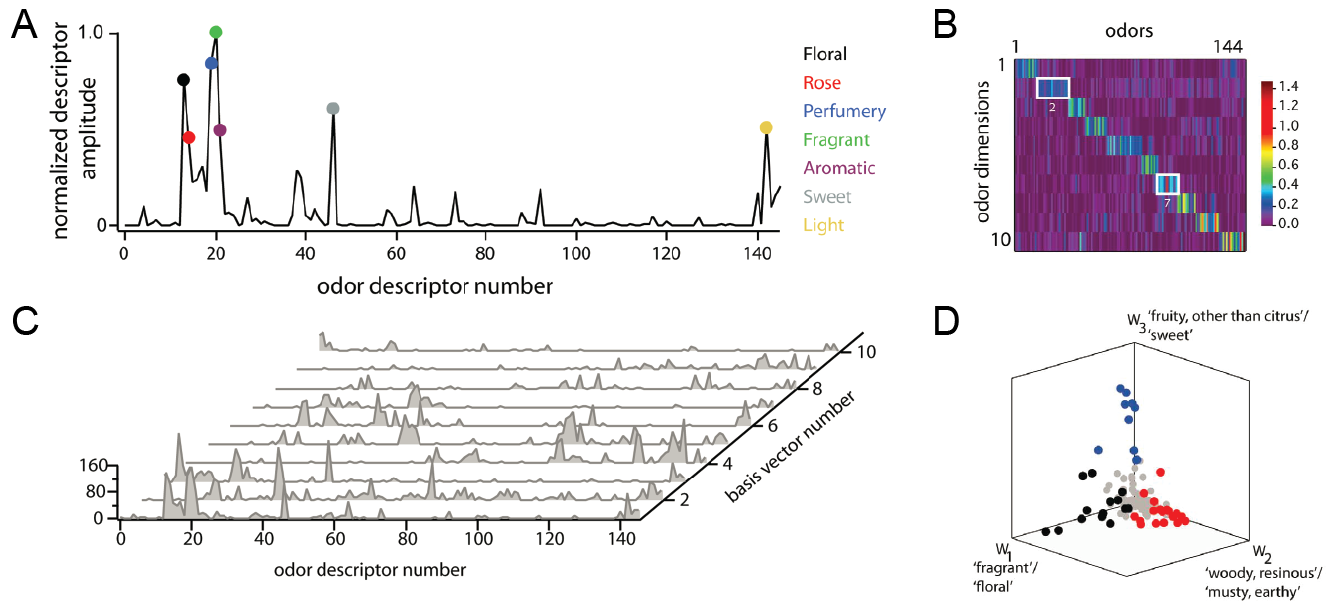
\includegraphics[width=\textwidth]{fig-rev1-olfaction}
    \caption{\ac{NMF} recovers a sparse and parts-based representation
    of olfactory perceptual space (reprinted from \cite{Castro2013}).
       \textbf{\emph{A}},
          Plot of normalized odor descriptor amplitude vs. odor descriptor number for
          the first basis function. Each point along the x-axis corresponds to a single
          odor descriptor, and the amplitude of each descriptor indicates the
          descriptor's relevance to the shown perceptual basis function.
          Colored circles show the 7 largest elements, with corresponding descriptors
          listed on the right.
       \textbf{\emph{B}},
          Waterfall plot of the 10 basis functions constituting \textbf{W}.
       \textbf{\emph{C}},
          Heat map of the coefficient matrix, \textbf{H},
          where each column of \textbf{H} corresponds to a different odor.
          Columns of \textbf{H} are normalized and sorted into groups defined by
          peak coordinate (1-10).
       \textbf{\emph{D}},
          Plot of all 144 odors in the dataset (each point is a column in \textbf{H})
          in the space spanned by the first three basis functions.
          Black, red, and blue points are those with peak coordinates in dimensions
          1, 2, and 3, respectively. Gray points are all remaining odors.}
	\label{fig:evidence-olfaction}
\end{figure}

Furthermore, \ac{NMF} recovered basis functions whose descriptors align
with perceptual dimensions highlighted in several previous analyses of odor space,
including but not limited to relative pleasantness (e.g., `fragrant`, `sickening`), 
and potential palatability (`woody, resinous', `chemical', `sweet', and `lemon').
Odors clustered predominantly along these axes
(Fig.~\ref{fig:evidence-olfaction}D), 
motivating the interpretation that odor space is organized 
by a relatively large number of independent qualities that apply categorically
\cite{Castro2013}.


\subsection*{NSC in the somatosensory cortex}

Of all of the sensory areas,
somatosensory cortex is among the best understood in terms of circuitry,
yet least understood in terms of sensory function
\cite{Ramirez2014}.
Spatiotemporal receptive fields indicate that individual neurons respond to a small number of stimulus dimensions, suggesting a role for dimensionality reduction in primary somatosensory cortex \cite{Ramirez2014}.
In an effort to elucidate the stimulus dimensions that individual neurons respond to,
Whiteway and Butts \cite{WhitewayButts2017} devised the \ac{RLVM},
a combination of nonlinear dimensionality reduction with nonnegativity constraints
that is closely related to \ac{NSC}.
When they applied the \ac{RLVM} to 
a two-photon imaging dataset of hundreds of simultaneously recorded neurons 
in mouse primary somatosensory cortex while the animal was performing
a tactile discrimination task,
they found basis functions that properly identified individual neurons.
Similar to the recorded neuronal responses, these basis functions were closely related
to both the tactile stimulation as well as 
nonstimulus aspects of the behavioral task.
Furthermore, \ac{RLVM} achieved a lower reconstruction error than other
linear dimensionality reduction techniques such as \textbf{\ac{PCA}}.

Similar to auditory cortex,
activity in somatosensory cortex can be extremely sparse
\cite{Jadhav2009,oconnor2010,Crochet2011},
and sparse coding models have successfully explained the response properties
of individual neurons in rat somatosensory cortex (e.g., \cite{Hafner2004}).
In addition, the presence of a topographically organized sensory `homunculus' 
in various species \cite{penfield1937,hari1993,petersen2007} 
suggests a possible parts-based representation scheme.


\subsection*{NSC in the retrosplenial cortex (RSC)}

In our own work, we found evidence that \ac{NSC} 
can explain response properties in \ac{RSC}, 
an area important for navigation and spatial memory 
\cite{Miller2014,Nelson2015,VannAggleton2009}.
Using a similar methodology to \cite{Beyeler2016},
we applied \ac{NMF}, with a sparsity constraint,
to parameterized behavioral variables extracted from electrophyisiological recordings
of \ac{RSC} neurons in the rat \cite{AlexanderNitz2015}
while the animal ran back and forth a W-shaped track
(for experimental details, see Supplementary Material).
As mentioned above, these behavioral variables included the animal's position, head direction, 
and movement direction (Fig.~\ref{fig:NMF|reconstruction}C).
The basis functions recovered by \ac{NMF} were then used to generate simulated responses
of model \ac{RSC} neurons according to Eq.~\ref{eqn:nsc-model-response},
and the simulated responses were compared to neuronal responses 
from the electrophysiological recordings.

We found that the population activity of these simulated neurons could be used to predict
the animal's location both with respect to the beginning of the route
(route-based reference frame)
and with respect to where the route was located within the room
(allocentric reference frame).
In addition, simulated neuronal activity could be classified into three broad categories,
with remarkably similar population statistics to rat \ac{RSC}:
1) responding to left and right turns on a specific position along the route,
2) responding to left and right turns regardless the position along the route,
and 3) exhibiting complex and robust firing patterns without turn sensitivity
(see Supplementary Material; also Fig.~\ref{fig:NMF|RSC}A, B).


\subsection*{Reinforcement-driven NSC in the basal ganglia}

\mikeNote{R1: To reach a broader audience, the authors should describe better the mechanisms of Hebbian and Anti-Hebbian plasticity in the Basal ganglia section.}
There is computational evidence 
for a reward-driven variant of \ac{NSC} in the basal ganglia, 
a cluster of deep forebrain nuclei that are involved in the 
processing of motor, associative, and limbic information
(for recent reviews see \cite{BarGad2003_Review,NelsonKreitzer2014}).
The basal ganglia connect most cortical areas to the frontal cortex through
a series of convergent and sparsely connected pathways \cite{schwab2015},
where signals from tens of millions of cortical neurons are projected
onto a $10 - 10,000$ fold smaller population of neurons in different subnuclei
of the basal ganglia \cite{BarGad2003_Review}.

The \ac{RDDR} model suggests that dimensionality reduction 
in the cortico-basal ganglia pathway is achieved via
a combination of Hebbian and anti-Hebbian learning rules
that are implemented by feedforward excitatory and lateral inhibitory
connections \cite{BarGad2000,BarGad2003_Review}.
A reinforcement signal modulates the Hebbian learning rule 
of the feedforward projections,
allowing the network to learn to extract input dimensions
that are associated with reward activity
while suppressing behaviorally irrelevant input dimensions.
Whereas the original \ac{RDDR} model was a neural-network based model
for performing \ac{PCA} \cite{BarGad2000},
later iterations incorporated nonnegativity constraints on the
connection weights that effectively transformed the model 
into an \ac{NMF} variant \cite{BarGad2003_Review}.

In addition to suggesting a role for lateral connectivity
in the basal ganglia,
the \ac{RDDR} model also advanced understanding of basal ganglia dysfunction
in movement-related disorders such as Parkinon's and Huntington's disease.
Through a series of simulations, Bar-Gad and colleagues \cite{BarGad2003_Review}
argued that focal lesions should have little effect on behavior,
because of the network's ability to reorganize connections,
whereas abnormal dopamine levels should significantly alter 
the reinforcement signal that controls the model's ability 
to discriminate behaviorally relevant input signals.
\mikeNote{R1: cliffhanger: Did Bergman and colleagues test their predictions for focal lesions? What would the authors expect?}


\subsection*{Potential for NSC in other regions of the brain}

In addition to the areas highlighted above,
there is increasing evidence that the essential components of \ac{NSC}
might be present in numerous brain regions 
not traditionally associated with the efficient encoding of information.

For example, there is evidence for sparse coding in the
cerebellum \cite{Marr1969,Schweighofer2001,Brunel2004},
\ac{PFC} \cite{Abeles1990,Fujisawa2008,Wei2015},
motor cortex \cite{Beloozerova2003,Kakei2003,BarthPoulet2012,Brecht2004},
hippocampus \cite{rolls2013,ThompsonBest1989,Poli2017,Wixted2014},
and the amygdala \cite{Bach2011}.
Similarly, there is evidence for dimensionality reduction in
\ac{PFC} \cite{Mante2013}
and motor cortex \cite{Graziano2009,Gallego2017}.
However, the intrinsically complex response properties of individual neurons
have defied a deep understanding of how these neurons contribute to behavior
\cite{churchland2007,Mante2013}.
For example, individual \ac{PFC} neurons typically encode multiple task-related signals
at once, including the animal's upcoming choice, the context,
and the strength of the sensory evidence \cite{Mante2013,Rigotti2013,Kobak2016}.
Future studies may show that key features of the population response in these regions
can be recovered by applying \ac{NSC} to their inputs.

Analogous to our modeling work in \ac{MSTd} \cite{Beyeler2016},
it might be possible to apply \ac{NSC} to other areas of the posterior parietal
cortex that are involved in multisensory heading perception.
Areas such as the \ac{VIP} and \ac{VPS} are also known to respond to optic flow,
but they increasingly respond to inertial vestibular stimulation as well
\cite{Chen2011}.
Although the degree of sparsity of the population code in \ac{VIP} and \ac{VPS} is not known,
the fact that neurons in these areas respond to mixtures of visual and vestibular
heading cues make them prime examples 
to be examined with an \ac{NSC} based modeling approach.

Elsewhere in parietal cortex, single neurons act as basis functions 
to represent the spatial configuration of objects 
with respect to multiple reference frames
(e.g., by transforming eye-centered to body-centered coordinates).
\cite{Poggio1990,PougetSejnowski1997,PougetSnyder2000}.
This is similar to the integration of multimodal heading cues mentioned above,
as well as to other associative areas such as \ac{RSC},
which demonstrates conjunctive coding of various spatial navigation cues
\cite{AlexanderNitz2015,Rounds2018}.
There is further evidence that actions are represented in parietal cortex
with respect to arbitrary and abstract reference frames, 
such as with respect to a planned route through an environment \cite{nitz2009parietal}.
From a theoretical standpoint, \ac{NSC} seems a good candidate to find an efficient,
reference-frame agnostic representation of various behaviorally relevant variables
\cite{LouieGlimcher2012,louie2015adaptive,andersen1997multimodal,BenHamed2003},
but future studies will have to address these issues step by step.

\section*{Discussion}
\label{sec:discussion}

That \ac{NSC} can explain and reproduce response properties 
observed in biological neurons 
may be an important clue as to how 
\revise{sensory and associative brain areas}
have evolved to parse and store information
in order to perceive the world and interact with it.
\mikeNote{This is indeed written in a very sensory-centric manner}
We offer three testable predictions of this theory:

First, we suggest that a variety of neuronal response properties
can be understood as an emergent property of efficient population coding 
based on dimensionality reduction.
Depending on input stimulus and task complexity,
we expect the dimensionality of the population code to be adjusted
according to the bias-variance dilemma
(Fig.~\ref{fig:nsc-bias-variance-dilemma}).
This point of operation might differ across brain areas---for example,
favoring neurons that respond to a small number of stimulus dimensions
in \ac{V1} \cite{OlshausenField1996},
but giving rise to mixed selectivity in higher-order brain areas
such as \ac{MSTd} \cite{Beyeler2016} and
\ac{RSC} \cite{Rounds2016,Rounds2018}.
% and \ac{PFC} \cite{Mante2013}.

Second, we predict that parts-based representations can explain
\acp{RF} of neurons in a variety of brain regions,
including but not limited to those brain areas discussed here. 
In agreement with the literature on basis function representations
\cite{PougetSejnowski1997,PougetSnyder2000,Poggio1990},
we expect parts-based representations
to be prevalent in regions where neurons
exhibit a range of tuning behaviors \cite{Beyeler2016},
display mixed selectivity \cite{Fusi2016,Eichenbaum2017},
or encode information in multiple reference frames 
\cite{AlexanderNitz2015,Rounds2016,Rounds2018}.

Third, where such representations occur, we expect the resulting
neuronal population activity to be relatively sparse,
in order to encode information both accurately and efficiently.
As noted above, sparse codes offer a trade-off between 
dense codes (where every neuron is involved in every context,
leading to great memory capacity but suffering from cross talk among neurons)
and local codes (where there is no interference, 
but also no capacity for generalization).
% \ac{NSC} explicitly discourages statistically inefficient representations,
% because strongly accounting for a rare observation at the expense of ignoring
% more common input components would result in an increased reconstruction error
% (see Eq.~\ref{eqn:nsc-cost-function}).


\subsection*{\revise{Potential for NSC in nonsensory areas of the brain}}

% \revise{Complex behaviors are accompanied by dynamic responses across cortical circuits.
% During decision-making, cortical activity reflects multiple processes including sensory inputs (Freedman and Assad, 2006; Meister et al., 2013), selection and integration of behaviorally-relevant information (Roitman and Shadlen, 2002), estimation and anticipation of reward (Bouret and Sara, 2004; Pratt and Mizumori, 2001), choice confidence (Kepecs et al., 2008) and recent trial history (Abrahamyan et al., 2016; Bichot and Schall, 1999; Manoach et al., 2007; Morcos and Harvey, 2016).} 

\mikeNote{Maybe fuse with model limitations?}
\mikeNote{R1: In the previous round of reviews, I already suggested that the authors’ model seems more appropriate for sensory areas, and that it may not apply to the motor system. Despite the changes to the paper, I think the paper would be clearer and perhaps more compelling that way. To be clear, I’m not arguing that the authors should complete remove non-sensory areas, but I think it should be a part of the Discussion ``Would these ideas apply to non-sensory areas?'' rather than of the core of the paper.}
\revise{In addition to the areas highlighted above,
there is increasing evidence that the essential components of \ac{NSC}
might be present in numerous brain regions 
not traditionally associated with the efficient encoding of information.}

\emilyNote{Should discussion of hippocampus go here?}

\revise{For example, there is evidence for sparse coding in the
cerebellum \cite{Marr1969,Schweighofer2001,Brunel2004},
\ac{PFC} \cite{Abeles1990,Fujisawa2008,Wei2015},
motor cortex \cite{Beloozerova2003,Kakei2003,BarthPoulet2012,Brecht2004},
hippocampus \cite{rolls2013,ThompsonBest1989,Poli2017,Wixted2014},
and the amygdala \cite{Bach2011}.
Similarly, there is evidence for dimensionality reduction in
\ac{PFC} \cite{Mante2013}
and motor cortex \cite{Graziano2009,Gallego2017}.
However, the intrinsically complex response properties of individual neurons
have defied a deep understanding of how these neurons contribute to behavior
\cite{churchland2007,Mante2013}.
For example, individual \ac{PFC} neurons typically encode multiple task-related signals
at once, including the animal's upcoming choice, the context,
and the strength of the sensory evidence \cite{Mante2013,Rigotti2013,Kobak2016}.
Future studies may show that key features of the population response in these regions
can be recovered by applying \ac{NSC} to their inputs.}

\revise{Analogous to our modeling work in \ac{MSTd} \cite{Beyeler2016},
it might be possible to apply \ac{NSC} to other areas of the posterior parietal
cortex that are involved in multisensory heading perception.
Areas such as the \ac{VIP} and \ac{VPS} are also known to respond to optic flow,
but they increasingly respond to inertial vestibular stimulation as well
\cite{Chen2011}.
Although the degree of sparsity of the population code in \ac{VIP} and \ac{VPS} is not known,
the fact that neurons in these areas respond to mixtures of visual and vestibular
heading cues make them prime examples 
to be examined with an \ac{NSC} based modeling approach.}

\revise{Elsewhere in parietal cortex, single neurons act as basis functions 
to represent the spatial configuration of objects 
with respect to multiple reference frames
(e.g., by transforming eye-centered to body-centered coordinates).
\cite{Poggio1990,PougetSejnowski1997,PougetSnyder2000}.
This is similar to the integration of multimodal heading cues mentioned above,
as well as to other associative areas such as \ac{RSC},
which demonstrates conjunctive coding of various spatial navigation cues
\cite{AlexanderNitz2015,Rounds2018}.
There is further evidence that actions are represented in parietal cortex
with respect to arbitrary and abstract reference frames, 
such as with respect to a planned route through an environment \cite{nitz2009parietal}.
From a theoretical standpoint, \ac{NSC} seems a good candidate to find an efficient,
reference-frame agnostic representation of various behaviorally relevant variables
\cite{LouieGlimcher2012,louie2015adaptive,andersen1997multimodal,BenHamed2003},
but future studies will have to address these issues step by step.}

\revise{Some studies indicate that the population code in \ac{PFC} and \ac{M1} may be
quite dense (as in Fig.~1A).
Dimensionality reduction studies suggest that in these areas population-wide features
are encoded by most neurons in the population \cite{Gallego2017,CunninghamYu2014,Kobak2016,Mante2013}.
Furthermore, \ac{M1} neurons tend to be active during most movements,
which argues against a very sparse activation.}
\mikeNote{This is word for word from R1. Need to revise.}



\subsection*{Potential neural mechanisms of NSC}

As a special case of efficient coding,
\mikeNote{R1: minimizing energy expenditure is not a clear requirement for the NSC model to be useful; maybe some areas try to maximize robustness or adaptability instead of miniziming energy expenditure. maybe that's why some areas are less sparse than others.}
\ac{NSC} possesses metabolic advantages by employing
sparse population codes.
To operate efficiently, it has been suggested that the brain might enforce 
geometrical and biophysical constraints on axonal wiring 
\cite{LaughlinSejnowski2003}.
In addition to reducing overall wiring length
\cite{Cherniak1994}, the brain might also aim to minimize local delays
by favoring a high degree of local connectivity
\cite{Chklovskii2002}.
\revise{If connectivity reflects} coding \cite{Clopath2010},
it would not be surprising to find that such ecological considerations
carry over into brain function,
favoring sparse population codes and neuronal representations that are
local in functional space (i.e., parts-based).
However, wiring cost is likely to be only one of many constraints 
on the brain connectome, perhaps supplementing competitive pressures
for hub-mediated information exchange between network modules
\cite{Rubinov2015}.

In addition, evidence suggests that Hebbian-like synaptic plasticity rules
allow neurons to perform statistical inference on their inputs
\cite{Nessler2009,Carlson2013,MorenoBoteDrugowitsch2015,Oja1982}.
One particular study demonstrated through a mathematical proof
that a certain form of \textbf{\ac{STDP}} in combination with 
homeostatic synaptic scaling (i.e., \ac{STDPH})
can approximate the \ac{NMF} algorithm
\cite{Carlson2013}.
Similar to Oja's rule \cite{Oja1982}, which was developed to stabilize 
rate-based Hebbian learning
(effectively resulting in principal component analysis),
Carlson and colleagues showed that synaptic scaling acts as a 
homeostatic mechanism to stabilize \ac{STDP}
(effectively resulting in \ac{NMF}).
Interestingly, we were able to apply these ideas to 
electrophysiologically recorded neuronal activity observed in the \ac{RSC}
of rats during a spatial navigation task (Fig.~\ref{fig:NMF|RSC}; for experimental details see Supplementary Material). Both \ac{STDPH} and \ac{NMF} were able to recover key  features such as encoding spatial reference frames (i.e., allocentric and route-centric firing patterns) and position discrimination by reducing the dimensionality of behavioral variables (e.g., velocity, head direction, position).
The neuronal and population responses from NMF and STDPH were comparable to the experimental findings \cite{AlexanderNitz2015}.
Furthermore, the \ac{STDPH} model contained a highly flexible and generalizable code
that could automatically encode new routes through the same environment
without retraining \cite{Rounds2018}.
However, more research is needed to elucidate any potential connection 
between \ac{NSC} and the many different synaptic plasticity rules 
commonly found across brain regions,
different stages in the life of an animal, and animal species
(e.g., \cite{Froemke2010,BCM1982}).
\mikeNote{R1:  Fig 8 is hard to interpret, what is the percent model error? Does this error reflect a ``movement prediction error''?}
\emilyNote{I think the reviewer doesn't realize it says "Pred. error" and not "P
ct. error"...}
\mikeNote{In that case, it would be good to spell it out in the figure}
\begin{figure}[h]
	\centering
	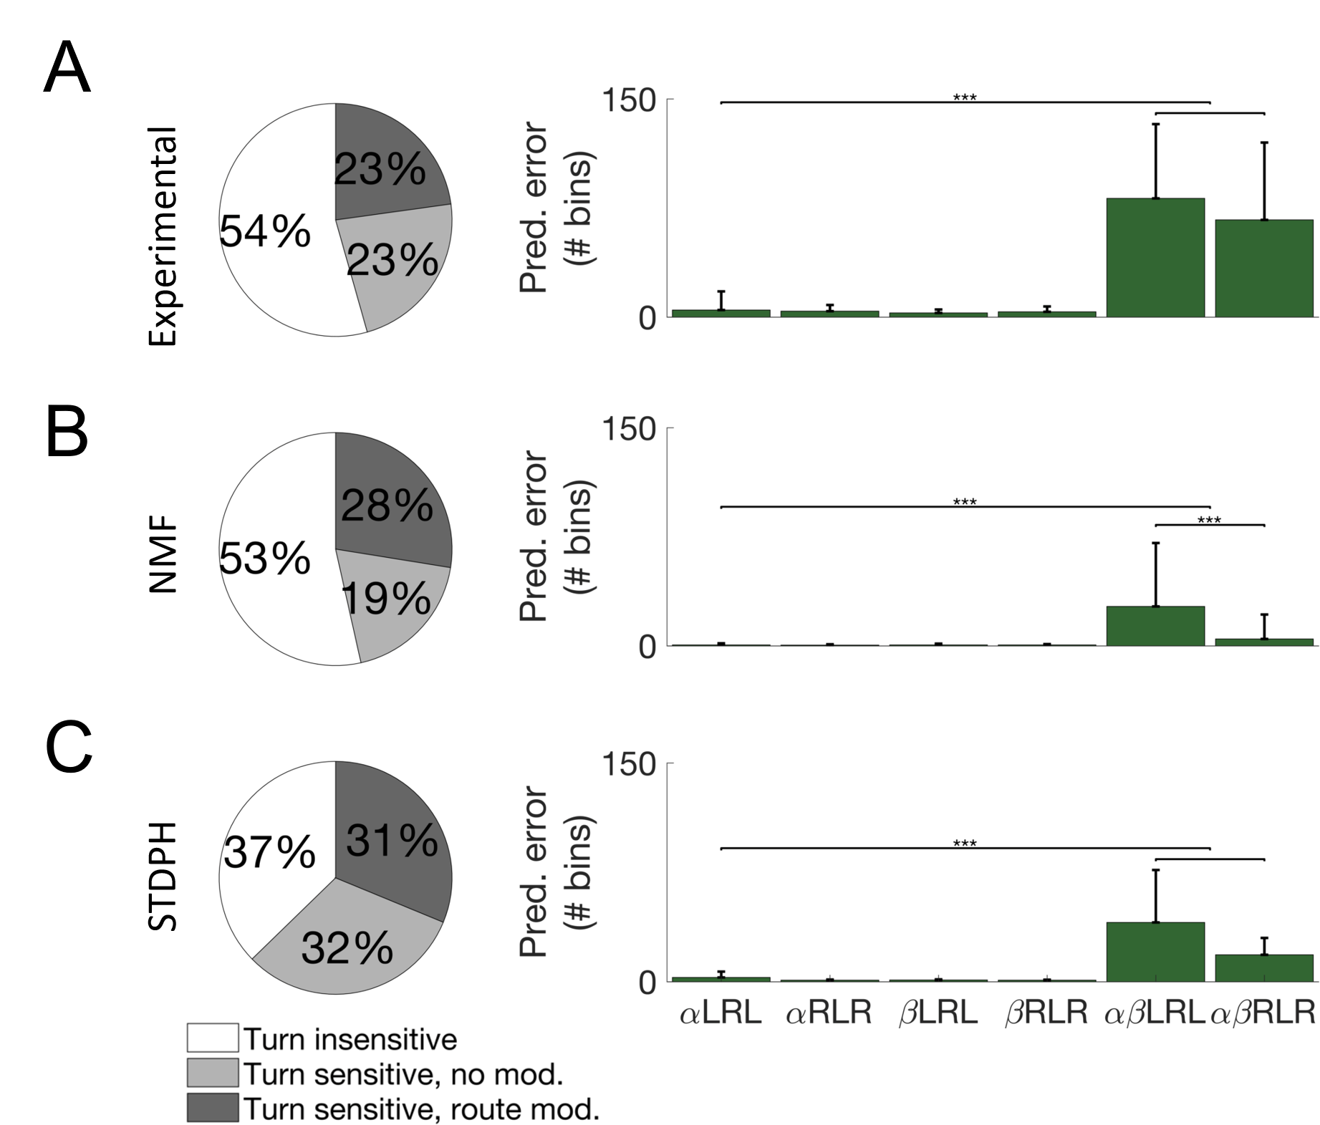
\includegraphics[width=0.95\textwidth]{fig-rev1-rsc}
    \caption{
    	Comparisons between recorded experimental data and two 
        computational models of rat \ac{RSC} suggest a functional 
        similarity between \ac{STDPH} and \ac{NMF}.
%         (adapted \revise{with permission} from \cite{Rounds2018}). 
        Using methods described in \cite{AlexanderNitz2015}, 
        we compared functional neuron type distributions (left column)
        and average \revise{movement} prediction errors (right column)
        observed \emph{in vitro} (\textbf{\emph{A}}) with those
        produced by each model (\textbf{\emph{B, C}}).
        Average error corresponded to correlation matrices 
        representing reconstructed position within a route. 
        For details, see Supplementary Materials.
        Separate positions of the W-shaped track are represented 
        by the symbols $\alpha$ and $\beta$. 
        Outbound and inbound runs were made up of 
        opposite turn sequences (left-right-left (LRL) 
        and right-left-right (RLR), respectively.
        Reconstructions between the track positions are represented by
        $\alpha \beta$.
	    \textbf{\emph{A}},
    		Experimental data from \cite{AlexanderNitz2015}.
        \textbf{\emph{B}},
            Simulated using NMF with sparsity constraints.
        \textbf{\emph{C}},
            Simulated by evolving \ac{STDPH} parameters 
            to fit experimental data \cite{BeyelerCarlsonChou2015,Carlson2014}.
    }
	\label{fig:NMF|RSC}
\end{figure} 


\subsection*{Model limitations}

% sparse single-neuron responses underlying dense population codes are a common feature of cortical representations at the level of firing rates

Although \ac{NSC} has proved useful in understanding
a variety of neuronal responses
as an emergent property of efficient population
coding based on dimensionality reduction and sparse coding,
there are some limitations to this theory.

First, it remains to be demonstrated whether \ac{NSC} in its current form
\mikeNote{This reads a bit like the new `will this apply everywhere' section}
can be extended to brain areas that require a dynamic process of information
gating, such as \ac{PFC} \cite{Mante2013,Rigotti2013,Kobak2016}
and motor cortex \cite{Vargas2010decoding,GrazianoAflalo2007}.
In these areas, diverse time courses across neurons have confounded
attempts to understand the basic encoding of decisions and movements.
\mikeNote{R1: when the authors mention the different time courses of neural activity across areas, maybe they want to mention that in motor areas activity seems to be well-represented by RNNs, whereas in visual areas feedforward nets seem to be better models?}
However, the same is true for the olfactory system,
where population activity traces out loops that are organized by stimulus
condition. In particular, the orientation of the loop 
is related to the odor identity,
and the size of the loop is related to the odor concentration
\cite{Broome2006}.
Nevertheless, a recent \ac{NSC} based study was able to elucidate perceptually
relevant dimensions in odor space \cite{Castro2013}.
Our hope is that similar studies applied to \ac{PFC} and motor cortex will
reveal similar insights into their population response properties.

\revise{Second, there is increasing evidence that several motor variables are encoded
throughout the brain, including early sensory areas 
\cite{CrochetPetersen2006,Pachitariu2015,Musall2018,Stringer2018}.
For example in the mouse, running modulates the gain of visual inputs 
\cite{Mineault2016,NiellStryker2010} 
and is critical for integration of visual motion \cite{Ayaz2013,Saleem2013}.
A potential explanation for these widespread effects is that 
certain movements reflect changes in the animal's internal state,
such as increased arousal during running \cite{NiellStryker2010}.
Another study found that stimuli and behavior 
were represented together in mouse \ac{V1} as a
mixed representation: there were not separate sets of neurons
encoding stimuli and behavioral variables, but each
neuron multiplexed a unique combination of sensory and
behavioral information \cite{Stringer2018}.
Interestingly, these results were not specific to visual cortex, but were seen across
wide regions of the mouse forebrain,
suggesting that neuronal activity in these areas is more than just an efficient
encoding of sensory stimuli.}

\revise{Third}, a practical limitation of dimensionality analyses in general
is that the apparent dimensionality of the population response changes
systematically with the complexity of the input stimulus
\cite{SpanneJorntell2015,Cowley2016,Mazzucato2016}.
For practical purposes, simulated models of neuronal circuitry are typically
built with far fewer units than the number of neurons in the real network.
By excluding input dimensions that are present in the brain,
one will implicitly guide the simulated model away from spurious interactions
that the real circuitry would have to handle.
As a result, the simulated model might underestimate 
the true complexity of the task.

\revise{Fourth}, the role of sparse coding in the brain has been questioned
\cite{SpanneJorntell2015,BarthPoulet2012}.
This is at least partly due to the wide variety of definitions of \revise{sparsity}
used in the literature:
In its widest possible theoretical sense,
a neuron population exhibits sparse activity if the average activation ratio
remains below 50\% for binary neurons 
or below 100\% for thresholded,
rate-based neurons \cite{SpanneJorntell2015}.
However, it is not surprising that different brain areas might employ
different degrees of sparsity.
\mikeNote{R1: These paragraphs are not very clear, starting with the authors’ definition of learning... Please rewrite}
Whereas learning can be extremely fast in a local code,
a network of `grandmother' cells suffers from low representational capacity.
As the degree of sparsity in the network decreases and the code gets denser,
representational capacity and fault tolerance 
(i.e., the capacity to handle neuronal noise or the loss of a subset of neurons)
improve,
but at the expense of a decrease in learning speed
\cite{Foldiak1990,SpanneJorntell2015}.
The optimal point of operation would therefore depend on the complexity of
the stimulus to be encoded or the task to be performed,
subject to constraints on the required speed of learning.
This point of operation might differ drastically across brain areas---for example,
favoring an extremely sparse code in \ac{V1}
\cite{OlshausenField1996},
but giving rise to a slightly denser code with 
greater representational capacity in higher-order visual areas
such as \ac{MSTd}, 
which could lead to compact and multifaceted encodings
of various perceptual variables
(see Discussion in \cite{Beyeler2016}).


\subsection*{Model alternatives}

Since \ac{NMF} is an integral part 
of Eq.~\ref{eqn:nsc-cost-function},
it is interesting to note that \ac{NSC} is tightly connected
to a number of unsupervised learning techniques,
such as $k$-means clustering,
an algorithm used to partition
$n$ observations into $k$ clusters
\cite{Ding2005}.
Due to its ability to decompose high-dimensional data into
sparse, interpretable factors, \ac{NMF} has become a 
widely used tool for the analysis of high-dimensional data,
with applications reaching far beyond
the field of computational biology
(for a recent review see \cite{Gillis2014}).

In addition to the tight connection 
to linear sparse coding and \ac{NMF}
\cite{EggertKorner2004},
\ac{NSC} is also intimately related to \textbf{\ac{ICA}},
a computational method for separating a multivariate signal
into additive, statistically independent subcomponents. 
As originally noted by Hoyer \cite{Hoyer2002},
if the fixed-norm constraint is placed on the rows of
\textbf{H} instead of the columns of \textbf{W},
Eq.~\ref{eqn:nsc-cost-function} can be directly interpreted as the joint
log-posterior of the basis functions and hidden components
in the noisy \ac{ICA} model \cite{HoyerHyvarinen2002}.
In order for this connection to hold,
the \ac{ICA} basis functions must be chosen to be nonnegative,
and the independent components must have 
exponential distributions \cite{Hoyer2002}.

Similarly, \ac{NSC} is closely related to compressed sensing
(for a recent review see \cite{GanguliSompolinsky2012}),
and a recent study has even suggested to combine the two
\cite{WangLi2010}.
Compressed sensing posits that neurons might implement 
\mikeNote{R1: recent paper from the Shenoy and Ganguli labs [13] that shows that this notion applies to M1 data}
dimensionality reduction by randomly projecting patterns of activity
into a lower-dimensional space,
simply by synaptically mapping $N$ upstream neurons to a downstream region
containing $M < N$ neurons. 
\revise{There is some evidence that this idea applies in some areas of the brain. For example, Trautmann et al. \cite{trautmann2017} applied random projection theory to data from three previous studies of motor area M1 and found that the reconstructed neural dynamics using this method yielded results quite similar to those derived from spike sorting.}
The theory of compressed sensing then provides the mathematical tools
to reconstruct the original space from the random projections.
\ac{NSC}, \ac{ICA}, and compressed sensing often make similar predictions
that only slightly differ in the nature of the basis function representation
necessary to achieve optimal reconstruction
(for details please refer to the Discussion of \cite{GanguliSompolinsky2012}).
For example, whereas \ac{ICA} emphasizes the statistical independence 
of unmixed sources
and compressed sensing requires basis function to be `maximally incoherent'
\cite{GanguliSompolinsky2012},
\ac{NSC} does not make any such assumptions
as long as the basis functions are nonnegative.

\section*{Acknowledgments}

Supported by the National Science Foundation (Award IIS-1302125) and the Washington Research Foundation Funds for Innovation in Neuroengineering and Data-Intensive Discovery (M.B.).
\section*{Glossary}
\label{sec:Glossary}

\begin{itemize}
\item \textbf{Allocentric reference frame} A spatial frame of reference that is defined with respect to a broader environment (e.g., one's location on a map). Hippocampal place cells are a textbook example of neurons that are anchored to an allocentric reference frame.

\item \textbf{Basis functions} A lower-dimensional set of linearly independent elements that can represent a high-dimensional input space given a weighted sum of these elements, where the weight of each element is defined by a separate hidden component. For example, according to Fourier analysis, sine and cosine are basis functions for the space of all continuous periodic functions.

\item \textbf{Dimensionality reduction} The process of reducing the dimensionality of a space to the lowest possible space that encapsulates the variance of the original data via feature extraction. In the case of neuronal firing rate patterns, this means representing all possible firing rate patterns in the brain region using the smallest possible subset of the neurons.

\item \textbf{Efficient coding} A theoretical model of sensory coding in the brain based on information theory \cite{Barlow1961,Attneave1954,Linsker1990}. The efficient coding hypothesis posits that sensory pathways can be understood as communication channels where neuronal spiking aims to maximize available channel capacity by minimizing the redundancy between representational units.

\item \textbf{Holistic representation} Representation of a stimulus space that does not rely on explicit representations of stimulus component parts.
For example, a house might be represented by the visual system as a set of house
`templates'. Although visual information from individual house components
(e.g., front door, windows, roof, etc.) would of course be included in the house
representation, that information would be not be contained in representational
packets corresponding to the parse of the house into these features.
Instead, houses would be recognized `all of a piece'.

\item \textbf{\Acf{ICA}} A computational method for decomposing multivariate data into additive components by assuming that the components are non-Gaussian signals and statistically independent from each other. Independent components differ from decorrelated components by the fact that the minimization includes higher-order and not only second-order statistics. A simple application of \ac{ICA} is the `cocktail party problem', where the underlying speech signals are separated from a sample data consisting of people talking simultaneously in a room.

\item \textbf{\Acf{NMF}} A computational method for decomposing multivariate data into additive components by constraining the components to be nonnegative. This constraint results in a parts-based representation, because it only allows additive, and not subtractive, combinations of subcomponents.

\item \textbf{Parts-based representation} Representation of a stimulus space
in terms of explicit representations of stimulus component parts.
For example, a house might be decomposed by the visual system into a set of doors,
windows, a roof, etc. The resulting representation of the house would consist of
representations of these parts, somehow linked together.

\item \textbf{\Acf{PCA}} A computational method for decomposing multivariate data into linearly uncorrelated components. \Ac{PCA} identifies an ordered set of orthogonal directions that captures the greatest variance in the data \cite{CunninghamYu2014}.

\item \textbf{Representational capacity} The number of recognizably different patterns of neuronal activity that a population of neurons can generate in a useful time interval \cite{Laughlin2001}.

\item \textbf{Route-centric reference frame} A spatial frame of reference that is defined with respect to a planned path through a broader environment. For example, neurons in some parts of the brain fire for a particular location in a route, even if the route is repositioned or reoriented in the broader environment \cite{nitz2009parietal}.

\item \textbf{Sparse coding} A population coding scheme for where activity is represented by the strong activation of a relatively small set of neurons. Sparse coding can be described as a trade-off between the benefits and drawbacks of dense and local codes \cite{Foldiak1990}. For example, the speed of learning of a local code is traded against the high representational capacity allowed under a dense code.

\item \textbf{Spike-timing dependent plasticity (STDP)} A Hebbian-inspired learning rule in which weight updates are computed based on the precise spike times of pre- and post-synaptic neurons that induce either long term potentiation or long term depression in the synapse, depending on whether the total pre-synaptic spike count preceded the total post-synaptic spike count, integrated over a critical temporal window.

\end{itemize}

\nolinenumbers
\bibliography{references}

% \appendix
% \linenumbers
% \include{S1-supplementary}

\end{document}